\documentclass{article}

\usepackage[utf8]{inputenc}
\usepackage[T1]{fontenc}
\usepackage{verbatim}
\usepackage{graphicx}

\title{Systemy operacyjne}

\begin{document}

\maketitle

\newpage \tableofcontents

\section{Funkcje systemów operacyjnych}

\subsection{Przykładowe funkcjl jakie pełni system operacyjny}
\begin{itemize}
    \item Planowanie, wykonywanie i nadzorowanie zadań
    \item Obsługa i kontrolowanie urządzeń
    \item Zarządzanie pamięcią masową
    \item Tworzenie mechanizmu umożliwiającego przechowywanie informacji (np. system plików)
    \item Stworzenie środowiska, dzięki któremu użytkownik może w sposób wygodny i wydajny zarządzać zadaniami
\end{itemize}

\subsection{Zastosowania rodzajów systemów operacyjnych}
\textbf{Wieloprocesorowe systemy operacyjne} - mają możliwość wykonywania wielu procesów, wykorzystując co najmniej dwa procesory lub kilka rdzeni procesora w systemie. \textbf{Planują i przydzielają zadania do dostępnych procesorów}, aby zapewnić mn.w. równe wykorzystanie zasobów oraz mn.w. równe obciążenie. Np: Windows, Linux, Unix.

\textbf{Systemy operacyjne czasu rzeczywistego} - \textbf{systemy czasu rzeczywistego muszą być w stanie obsłużyć zdarzenia w określonym czasie}. Twarde systemy czasu rzeczywistego są systemami w których operacje muszą być wykonane bezwzględnie w określonym czasie (systemy kontroli produkcji, systemy bezpieczeństwa, systemy wojskowe, systemy lotnicze, systemy medyczne). Miękkie systemy czasu rzeczywistego są systemami w których wykonanie operacji z niepożądanym opóźnieniem, nie powoduje poważnych strat (systemy multimedialne, systemy rozrywkowe, systemy telekomunikacji, systemy zarządzające budynkiem). Np: FreeRTOS, VxWorks, QNX, eCos.

\newpage\textbf{Systemy operacyjne dla komputerów mainframe} - są w stanie obsługiwać znacznie więcej urządzeń wejścia-wyjścia (np. mogą obsługiwać ponad 1000 dysków). Mogą wykonywać wiele zadań jednocześnie i zazwyczaj oferują trzy usługi: \textbf{przetwarzania wsadowe, przetwarzanie transakcji oraz podział czasu}.

\begin{itemize}
\item \textbf{Systemy wsadowe} są systemami, które wykonują zadania automatycznie i sekwencyjnie, bez interakcji z użytkownikiem. Obecnie są stosowane np. w przetwarzaniu transakcji finansowych, w generowaniu raportów sprzedaży.
\item \textbf{Systemy przetwarzania transakcji} służą do przetwarzania operacji, które prowadzą do zmiany zasobów oraz obsługują dużą liczbę żądań. Obecnie przykładowe zastosowania: przetwarzanie czeków, systemy rezerwacji.
\item \textbf{Systemy z podziałem czasu} pozwalają wielu zdalnym użytkownikom na jednoczesne uruchomienie zadań na komputerze.
\end{itemize}
Np: OS/390, BS2000.

\textbf{Systemy operacyjne dla serwerów} - dostosowane do działania na serwerach, czyli komputerach lub innych narzędziach, które \textbf{pozwalają na dostarczenie zasobów lub współdzielenie usług, dla wielu użytkowników jednocześnie, przez sieć}. Np: Linux, Windows Server, OS X Server, FreeBSD, Solaris.

\textbf{Systemy operacyjne dla komputerów osobistych} - dostosowane do działania na komputerach osobistych. Większość systemów operacyjnych dla komputerów oferuje wygodny interfejs graficzny dla użytkownika, wygodne zarządzanie plikami i folderami, uruchamianie programów oraz umożliwia dostęp do internetu. Np: Linux, Windows, macOS, FreeBSD.

\textbf{Systemy operacyjne dla komputerów przenośnych} - dostosowane do działania na komputerach przenośnych, tj. smartfony, tablety, notebooki.

\textbf{Systemy operacyjne wbudowane} - dostosowane do działania na urządzeniach wbudowanych, czyli urządzeniach elektronicznych, które są przeznaczone do pełnienia konkretnych zadań lub funkcji. Systemy wbudowane \textbf{nie wymagają instalowania aktualizacji i są odporne na szkodliwe oprogramowanie - całe oprogramowanie jest zapisane w pamięci tylko do odczytu}. Np: FreeRTOS, VxWorks, QNX, MicroC/OS.

\newpage\subsection{Praca komputera w trybie jądra i trybie użytkownika}
Większość komputerów pracuje w dwóch trybach:
\begin{itemize}
    \item \textbf{tryb jądra} (inaczej tryb nadzorcy) (ang. supervisor mode) - można uruchomić każdą instrukcję, którą komputer jest zdolny uruchomić.
    \item \textbf{tryb użytkownika} - można uruchomić tylko pewien podzbiór instrukcji, które komputer jest zdolny uruchomić.
\end{itemize}
System operacyjny pracuje w trybie jądra.

\section{Systemy plików}
\subsection{System plików}
\textbf{System plików} to metoda i struktura organizacji danych na nośnikach. Umożliwia on:
\begin{itemize}
    \item przechowywanie danych
    \item utworzenie struktury katalogów ułatwiającą szeregowanie plików
    \item udostępnienie przechowywanych danych przy pomocy ścieżek
    \item zarzadzanie uprawnieniami dostępu do plików i katalogów
    \item tworzenie kopii zapasowych i umożliwienie odzyskiwania danych
\end{itemize}

\subsection{Przykładowe systemy plików}
\begin{itemize}
    \item \textbf{Ext4} - utworzony dla systemów Linux.
    \item \textbf{NTFS} - utworzony dla systemów Windows.
    \item \textbf{FAT} - utworzony dla systemów Windows.
    \item \textbf{UFS} - utworzony dla systemów Unix.
    \item \textbf{HFS+} - utworzony dla systemów macOS.
    \item \textbf{APFS} - utworzony dla systemów macOS.
\end{itemize}

\newpage\subsection{Zastosowania plików w systemie Linux}
\textbf{Plik zwykły} - służy do przechowywania danych tekstowych, binarnych, obrazów, dźwięków, filmów, itp.

\textbf{Katalog} - służy do przechowywania plików i innych katalogów. (katalogi organizują strukturę systemu plików)

\textbf{Plik specjalny} - służy do interakcji z urządzeniami wejścia-wyjścia.
\begin{itemize}
    \item \textbf{Urządzenie blokowe} - pliki dla urządzenia obsługujące dane o stałym rozmiarze, tj. dyski twarde, pendrive, karta graficzna.
    \item \textbf{Urządzenie znakowe} - pliki dla urządzenia obsługujące dane o zmiennej długości, tj. klawiatura, mysz, drukarka.
\end{itemize}

\textbf{dowiązanie} (ang. link) - służy do przechowywania odnośnika do pliku lub katalogu.
\begin{itemize}
    \item \textbf{dowiązanie twarde} - odnośnik do pliku lub katalogu, wskazuje na to samo miejsce w pamięci masowej. Po usunięciu pliku, dowiązanie nadal pozostaje aktywne
    \item \textbf{dowiązanie symboliczne} - zawiera jedynie ścieżkę do pliku lub katalogu. Po usunięciu pliku, na który wskazuje, dowiązanie może zostać nieaktywne.
\end{itemize}

\textbf{gniazdo} (ang. socket) - służy do komunikacji międzyprocesowej. Stosowane głównie w oprogramowaniu sieciowym 

\textbf{potok nazwany} (ang. named pipe) - służy do komunikacji międzyprocesowej na zasadzie potoku. Stosowane głównie na tym samym komputerze.

\subsection{Zastosowanie systemowych katalogów w systemie Linux}
\begin{itemize}
    \item \textbf{/} - katalog główny, korzeń systemu plików.
    \item \textbf{/bin} - katalog zawierający pliki wykonywalne dostępne dla wszystkich użytkowników.
    \item \textbf{/boot} - katalog zawierający pliki niezbędne do uruchomienia systemu.
    \item \textbf{/dev} - katalog zawierający pliki specjalne reprezentujące urządzenia.
    \item \textbf{/etc} - katalog zawierający pliki konfiguracyjne, administracyjne i inne pliki systemowe dla systemu lokalnego.
    \item \textbf{/home} - przechowuje katalogi domowe dla użytkowników.
    \item \textbf{/lib} - katalog zawierający współdzielone biblioteki systemowe.
    \item \textbf{/lost+found} - przechowuje pliki uszkodzone lub zgubione (takie, które nie mają przypisanego katalogu).
    \item \textbf{/mnt} - przeznaczony do tymczasowego montowania systemów plików.
    \item \textbf{/opt} - katalog zawierający opcjonalne pakiety oprogramowania.
    \item \textbf{/proc} - katalog zawierający informacje o stanie aktualnie działających procesów.
    \item \textbf{/root} - katalog domowy dla użytkownika root.
    \item \textbf{/run} - system plików tmpfs (system plików w pamięci RAM), który zawiera pliki i katalogi używane przez różne procesy.
    \item \textbf{/sbin} - katalog zawierający pliki wykonywalne, które wykonują czynnności administracyjne.
    \item \textbf{/sys} - przechowuje informacje potrzebne do zarządzania urządzeniami systemu operacyjnego.
    \item \textbf{/tmp} - katalog zawierający pliki tymczasowe.
    \item \textbf{/usr} - katalog zawierający pliki (programy, biblioteki, pliki konfiguracyjne) przeznaczone dla użytkowników systemu.
    \item \textbf{/var} - katalog zawierający pliki, które często ulegają zmianie, tj. logi, kopie zapasowe, maile. 
\end{itemize}

\subsection{Prawa dostępu do plików w systemie Linux}
Systemy typu Unix umożliwiają określenie praw dostępu dla:
\begin{itemize}
    \item właściciela pliku lub katalogu;
    \item grupy do której plik lub katalog należy;
    \item pozostałych użytkowników, którzy nie są właścicielem, ani nie należą do grupy pliku lub katalogu.
\end{itemize}
Standardowe prawa dostępu:
\begin{itemize}
    \item \textbf{prawo czytania} (ang. read) pozwala na odczyt pliku lub zawartości do katalogu;
    \item \textbf{prawo zapisu} (ang. write) pozwala na zapisanie lub modyfikacje pliku lub zmianę zawartości katalogu;
    \item \textbf{prawo wykonywania} (ang. execute) pozwala na wykonanie (uruchomienie) pliku (tyczy się skryptów, albo programów) lub otwierania katalogu.
\end{itemize}

Systemy Unix udostępniają możliwość korzystania z rozszerzonych praw dostępu, takich jak:

\begin{itemize}
    \item \textbf{Bit SUID} (ang. set user ID) - stosowany głównie do plików wykonywalnych. Powoduje, że program dziedziczy uprawnienia właściciela, co umożliwia mu obsługę danych, do których ma dostęp administrator. Jest ustawiany jako prawo wykonania dla użytkownika (właściciela) (s).

    \item \textbf{Bit SGID} (ang. set group ID) - stosowany głównie do katalogów, plików wykonywalnych i skryptów. Powoduje, że nowo utworzony plik lub katalog ma przypisaną grupę katalogu, w którym został utworzony. Jest ustawiany jako prawo wykonania dla grupy (s).

    \item \textbf{Bit lepkości} (ang. sticky bit) - stosowany głównie do katalogów. Powoduje, że użytkownicy, którzy nie są właścicielami ani nie należą do grupy katalogu, nie mogą usuwać zawartości katalogu, której nie są właścicielami, nawet jeśli posiadają prawo zapisu. Jest ustawiany jako prawo wykonania dla innych użytkowników (t).
\end{itemize}

\subsection{chmod}
\begin{table}[ht]
\centering
\begin{tabular}{|c|c|c|c|c|c|c|c|c|}
\hline
\multicolumn{3}{|c|}{\textbf{Właściciel}} & \multicolumn{3}{c|}{\textbf{Grupa}} & \multicolumn{3}{c|}{\textbf{Inni}} \\
\hline
\textbf{r} & \textbf{w} & \textbf{x} & \textbf{r} & \textbf{w} & \textbf{x} & \textbf{r} & \textbf{w} & \textbf{x} \\
\hline
4 & 2 & 1 & 4 & 2 & 1 & 4 & 2 & 1 \\
\hline
\end{tabular}
\end{table}
\begin{table}[ht]
    \centering
    \begin{tabular}{|c|c|c|}
    \hline
    \textbf{u} & \textbf{g} & \textbf{o} \\
    \hline
    \textbf{s} & \textbf{s} & \textbf{t} \\
    \hline
    4 & 2 & 1 \\
    \hline
\end{tabular}
\end{table}

Modyfikacja przy pomocy notacji symbolicznej:
\begin{itemize}
    \item \texttt{chmod u=rw direct} - przypisuje właścicielowi prawa do odczytu i zapisu.
    \item \texttt{chmod u+rx file.sh} - dodaje właścicielowi prawa do zapisu i wykonania.
    \item \texttt{chmod go-rwx file.c} - odbiera wszystkie prawa grupie i pozostałym użytkownikom.
    \item \texttt{chmod a+r file.txt} - dodaje wszystkim prawa do odczytu.
    \item \texttt{chmod u+s plik} - dodaje bit SUID dla właściciela pliku.
    \item \texttt{chmod u-s plik} - odbiera bit SUID dla właściciela pliku.
    \item \texttt{chmod g+s katalog} - dodaje bit SGID dla grupy katalogu.
    \item \texttt{chmod g-s katalog} - odbiera bit SGID dla grupy katalogu.
    \item \texttt{chmod o+t katalog} - dodaje bit lepkości dla innych użytkowników.
    \item \texttt{chmod o-t katalog} - odbiera bit lepkości dla innych użytkowników.
    \item \texttt{chmod 3755 katalog} przypisuje bit SGID (2) i bit lepkości (1) (2+1=3)
\end{itemize}

\subsection{umask}
\textbf{umask} - umożliwia określenie domyślnych praw dla nowo tworzonych plików i katalogów.
Domyślne prawa dla plików to 666, a dla katalogów 777. Umask określa, które prawa zostaną odjęte od tych wartości.
\begin{table}[ht]
\centering
\begin{tabular}{|c|c|c|}
\hline
\textbf{Umask} & \textbf{Prawa dla plików} & \textbf{Prawa dla katalogów} \\
\hline
000 & 666 & 777 \\
\hline
022 & 644 & 755 \\
\hline
XYZ & 666 - X*100 - Y*10 - Z & 777 - X*100 - Y*10 - Z \\
\hline
\end{tabular}
\end{table}

\subsection{Deskryptory i potoki}
\textbf{Deskryptor pliku} to identyfikator mający na celu identyfikację źródła pobierania i wysyłania danych.

\begin{itemize}
    \item \textbf{0} - standardowy strumień wejścia (\texttt{stdin}) to miejsce, z którego program pobiera dane (np. pobrane z klawiatury).
    \item \textbf{1} - standardowy strumień wyjścia (\texttt{stdout}) to miejsce, gdzie program może wysłać dane (np. do drukarki, wyświetlane na ekran).
    \item \textbf{2} - standardowy strumień błędów (\texttt{stderr}) to miejsce, gdzie program może wysłać informacje o błędach (np. na ekran).
\end{itemize}

\textbf{Przekierowanie} to mechanizm umożliwiający zmianę miejsca z którego
są pobierane lub przesyłane dane.
Operatory przekierowania:
\begin{itemize}
    \item \texttt{polecenie < plik} - przekierowanie standardowego wejścia.
    \item \texttt{polecenie > plik} - przekierowanie standardowego wyjścia (nadpisanie).
    \item \texttt{polecenie >> plik} - przekierowanie standardowego wyjścia (dopisanie).
    Powyższe operatory mogą być poprzedzone numerem deskryptora.
    \item \texttt{polecenie \&> plik} - przekierowanie standardowego wyjścia i błędów (nadpisanie).
    \item \texttt{polecenie \&>> plik} - przekierowanie standardowego wyjścia i błędów (dopisanie).
\end{itemize}
Operatory zarządzające deskryptorami:
\begin{itemize}
    \item \texttt{>\& numer} - przekierowanie wyjścia na deskryptor o podanym numerze.
    \item \texttt{<\&-} - zamknięcie standardowego wejścia.
    \item \texttt{>\&-} - zamknięcie standardowego wyjścia.
    \item \texttt{<\& numer} - pobiera wejście z deskryptora o podanym numerze.
    \item \texttt{numer <> plik} - otwiera deskryptor o podanym numerze i przypisuje do niego plik.
\end{itemize}

\textbf{Potok} (ang. pipe) służy do przekazywania standardowego wyjścia jednego polecenia na standardowe wejście innego polecenia.

Operatory potoków:
\begin{itemize}
    \item{\texttt{polecenie1 | polecenie2}} - przekazuje standardowe wyjście polecenia1 na standardowe wejście polecenia2.
    \item \texttt{polecenie1 |\& polecenie2} - przekazuje standardowe wyjście i błędy polecenia1 na standardowe wejście polecenia2.
\end{itemize}

\textbf{FIFO}, inaczej potok nazwany (ang. named pipe) to specjalny rodzaj pliku, który umożliwia komunikację między procesami.
Przykłady użycia FIFO:
\begin{itemize}
    \item \textbf{Utworzenie FIFO}: \texttt{mkfifo myfifo}
    \item \textbf{FIFO jako wyjście dla programu}: \texttt{ls > myfifo}
    \item \textbf{FIFO jako wejście dla programu}: \texttt{cat < myfifo}
    \item \textbf{Oczekiwanie na dane w FIFO}: \texttt{cat myfifo}
\end{itemize}

\section{Powłoki}
\subsection{Powłoka}
\textbf{Powłoka} (ang. shell) to interpreter poleceń oraz język programowania, który pozwala na tworzenie skryptów.

\textbf{Podpowłoka} (ang. subshell), to proces, który jest tworzony przez bieżącą powłokę i symuluje pracę powłoki. W podpowłoce wykonywane są zadania oraz przekazywane są informacje odnośnie wyjścia i błędów do powłoki.

\textbf{Zmienne środowiskowe} są przechowywane i zarządzane przez powłokę. Zmienne środowiskowe są dostępne dla wszystkich procesów potomnych.

\subsection{Przykładowe rodzaje powłok}
Pierwsza \textbf{powłoka sh} (Bourne Shell) dla systemu Unix Version 7, została stworzona przez Stephena Bourne’a w latach siedemdziesiątych. Wprowadziła ona wiele koncepcji w dziedzinie skryptów, poleceń i zarządzania systemem Unix.

Powłoki \textbf{kompatybilne z sh:}
\begin{itemize}
    \item \textbf{Bash} (Bourne Again Shell)
    \item \textbf{Dash} (Debian Almquist Shell)
    \item \textbf{Ksh} (Korn Shell)
\end{itemize}

\newpage Powłoki \textbf{niekompatybilne z sh:}
\begin{itemize}
    \item \textbf{Csh} (C Shell)
    \item \textbf{Fish} (Friendly Interactive Shell)
\end{itemize}

Powłoki systemu Windows:
\begin{itemize}
    \item \textbf{Cmd} (Command Prompt)
    \item \textbf{PowerShell}
    \item \textbf{WSL} (Windows Subsystem for Linux)
\end{itemize}

\subsection{Zastosowanie zmiennych środowiskowych}
Przykładowe zmienne środowiskowe:
\begin{itemize}
    \item \textbf{HOME} - ścieżka do katalogu domowego użytkownika.
    \item \textbf{PATH} - ścieżka do katalogów, w których znajdują się pliki wykonywalne.
    \item \textbf{PWD} - ścieżka do katalogu roboczego.
    \item \textbf{USER} - nazwa użytkownika.
    \item \textbf{LANG} - ustawienia językowe.
    \item \textbf{SHELL} - ścieżka do powłoki.
    \item \textbf{IFS} - separator pól (domyślnie spacja).
    \item \textbf{PS1} - znak zachęty.
    \item \textbf{PS2} - wtórny znak zachęty.
\end{itemize}

\subsection{Zastosowanie plików startowych i konfiguracyjnych}
Pliki startowe zawierają informacje niezbędne do zainicjowana pracy powłoki. Powłoka wykonuje pliki startowe kiedy jest uruchamiana.
\begin{itemize}
    \item \textbf{Plik \texttt{/etc/profile}} - plik wykonywany jako pierwszy podczas logowania - zawiera ustawienia dla wszystkich użytkowników np. zmienne środowiskowe
    \item \textbf{Plik \texttt{/etc/profile.d}} - katalog, w którym znajdują się skrypty konfiguracyjne, które są uruchomiane po wykonaniu.
    \item \textbf{Plik \texttt{\textasciitilde/.bash\_profile, \textasciitilde/.bash\_login, \textasciitilde/.profile}} - pliki, które są wykonywane po wykonaniu pliku \texttt{/etc/profile} - zawierają ustawienia dla indywidualnych użytkowników (np. mogą modyfikować globalne ustawienia).
    \item \textbf{Plik \texttt{\textasciitilde/.bash\_logout}} - polecenia wykonywane podczas wylogowywania, np. usuwanie plików tymczasowych.
    \item \textbf{Plik \texttt{/etc/bashrc}} - uruchamiany za każdym razem, kiedy uruchamiana jest nowa sesja powłoki, np. poprzez terminal - zawiera ustawienia dla interaktywnych sesji powłoki dla wszystkich użytkowników.
    \item \textbf{Plik \texttt{\textasciitilde/.bashrc}} - wykonywany po wykonaniu pliku /etc/bashrc - zawiera ustawienia dla interaktywnych sesji powłoki dla indywidualnych użytkowników.
\end{itemize}

\subsection{Zarządzanie operatorami logicznymi interpretera poleceń}
Operatory logiczne:
\begin{itemize}
    \item \textbf{||} - operator alternatywy (OR) - wykonuje kolejne polecenia, jeśli poprzednie zakończyły się niepowodzeniem.
    \item \textbf{\&\&} - operator koniunkcji (AND) - wykonuje kolejne polecenia, jeśli poprzednie zakończyły się sukcesem.
\end{itemize}

Inne operatory:
\begin{itemize}
    \item \textbf{;} - operator sekwencji - wykonuje kolejne polecenia niezależnie od wyniku poprzednich.
    \item \textbf{\&} - operator tła - uruchamia polecenie w tle.
\end{itemize}

\section{Systemy komputerowe}
\subsection{System komputerowy}
\textbf{System komputerowy} to układ współpracujących ze sobą dwóch składowych: sprzętu komputerowego (ang. hardware) oraz oprogramowania (ang. software).

Warstwy systemu komputerowego:
\begin{itemize}
    \item \textbf{Sprzęt komputerowy} - to wszystkie elementy fizyczne, które tworzą system komputerowy.
    \item \textbf{System operacyjny} - to oprogramowanie, które zarządza zasobami sprzętowymi oraz umożliwia korzystanie z komputera.
    \item \textbf{Programy narzędziowe} - wspomagają zarządzanie zasobami sprzętowymi oraz usprawniają oprogramowanie systemowe.
    \item \textbf{Programy użytkowe} - rozwiązują problemy zadane przez użytkownika (programy obliczeniowe, algorytmy)
    \item \textbf{Użytkownicy} - ludzie, urządzania lub inne podmioty, które realizują zadania przy pomocy programów użytkowych
\end{itemize}

\subsection{Oprogramowanie urządzeń wejścia-wyjścia}
Oprogramowanie związane z urządzeniami wejścia-wyjścia przeważnie jest zorganizowane w warstwach:
\begin{itemize}
    \item \textbf{Procedury obsługi przerwania} - \textbf{przerwanie} to działanie za pomocą którego zewnętrze układy sygnalizują zajście jakiegoś zdarzenia i żądają określonego działania. Przerwania powodują wstrzymanie wykonywania programu, wywołanie procedury, która wykonuje określoną czynność i na koniec wydaje instrukcję powrotu do wykonywanego programu.
    \item \textbf{Sterowniki urządzeń} - oprogramowanie odpowiedzialne za komunikację między urządzeniem a pozostałymi elementami systemu komputerowego.
    \item \textbf{Oprogramowanie niezależne od urządzenia} - oprogramowanie działające na poziomie systemu operacyjnego, które ma na celu dostarczenie wspólnego interfejsu dla różnych urządzeń (buforowanie, raportowanie, przydzielanie zwolnienia urządzeń).
    \item \textbf{Oprogramowanie poziomu użytkownika} - oprogramowanie działające na poziomie aplikacji użytkownika, które komunikują się z urządzeniami wejścia-wyjścia za pośrednictwem interfejsów dostarczanych przez warstwę oprogramowania niezależnego od urządzania (wyświetlenie na ekran, pobieranie danych).
\end{itemize}

\subsection{Procesor}
\textbf{Procesor} (CPU, ang. Central Processing Unit) jest układem odpowiedzialnym za sterowanie innymi układami lub elementami np. komputera.
Podstawowe elementy procesora:
\begin{itemize}
    \item \textbf{Rdzenie} - wykonują instrukcje programu i zawierają między innymi:
    \begin{itemize}
        \item \textbf{Układ sterowania} - kontroluje pracę procesora i wytwarza sygnały potrzebne do pracy z niektórymi elementami komputera. 
        \item \textbf{Arytmometr} (ALU) - służy do wykonywania operacji arytmetycznych, logicznych, przesunięć bitowych itp
        \item \textbf{Rejestry} - przechowują dane i wyniki.
    \end{itemize}
    \item \textbf{Pamięć podręczna Cache} - przechowuje ostatnio przetwarzane dane, co poprawia szybkość dostępu do informacji, które mają zostać ponownie wykorzystane.
    \item \textbf{Wewnętrzne szyny} - łączą elementu procesora z innymi elementami. które mają zostać ponownie wykorzystane.
\end{itemize}

\subsection{Pamięci ROM i RAM}
\textbf{Pamięć ROM} (ang. Read Only Memory) pamięć tylko do odczytu, która jest odporna na spadki napięcia. Zapisuje się na niej informacje, niezbędne do rozruchu urządzenia oraz dotyczące elementów budowy komputera (np. porty dysku).

\textbf{Pamięć RAM} (ang. Random Access Memory) pamięć operacyjna, która
przechowuje informacje odnośnie aktualnie przetwarzanych programów. Procesor współpracuje z pamięcią operacyjną, która przechowuje różne dane, instrukcje programów itp. stosując jednobajtowe komórki pamięci oraz ich numery adresów.

\subsection{Mechanizmy zarządzania pamięcią operacyjną}
\textbf{Przestrzeń adresowa} to zbiór wszystkich dopuszczalnych adresów w pamięci.
\begin{itemize}
    \item \textbf{przestrzeń fizyczna} - zbiór fizycznych adresów przekazanych do układów pamięci głównej.
    \item \textbf{przestrzeń logiczna} - zbiór adresów generowanych przez procesor w kontekście realizowanego zadania. \textbf{Adres logiczny} identyfikuje komórkę pamięci na poziomie kodu maszynowego w kontekście realizowanego zadania.
\end{itemize}
Procesory korzystają z \textbf{pamięci wirtualnej}. Mechanizm zarządzania pamięcią wirtualną polega na tym, że zadanie korzysta z obszaru pamięci mając wrażenie że korzysta z ciągłego obszaru, chodź w rzeczywistości \textbf{pamięć fizyczna może być pofragmentowana i nieciągła}. Możliwa jest też wymiana z pamięcią na dysku.

Procesor realizując zadanie korzysta z \textbf{mechanizmu segmentacji}, co oznacza, że pamięć jest dzielona na segmenty, które pełnią określone przeznaczenie.

W systemach wieloprocesowych procesor przechowuje \textbf{selektory w rejestrach segmentowych}, które \textbf{opisują własności początkowych adresów segmentów}. Budowa selektora:
\begin{table}[ht]
\centering
\begin{tabular}{|c|c|c|}
    \hline
    \textbf{Indeks} & \textbf{TI} & \textbf{RPL} \\
    \hline
\end{tabular}
\end{table}

\textbf{Deskryptor} to struktura, która \textbf{zawiera informacje dotyczące pewnego zasobu lub segmentu pamięci}. Deskryptor może zawierać informacje tj. \textbf{prawa dostępu, adres bazowy, rozmiar, typ zasobu itp}. \textbf{Tablica deskryptorów} to struktura, która przechowuje deskryptory. Tablica deskryptorów jest tworzona w pamięci operacyjnej i jest zarządzana przez system operacyjny (jest często tworzona i używana w systemach komputerowych, które korzystają z segmentacji pamięci). Tablica deskryptorów jest przydzielana każdemu procesowi oraz istnieje tablica deskryptorów, która definiuje opisy segmentów pamięci. Tablica deskryptorów może zawierać informacje odnośnie numeru deskryptora pliku. System operacyjny przydziela numer deskryptora (przeważnie od 3 wzwyż) podczas otwarcia pliku lub innego zasobu wejścia/wejścia. Istnieją stałe numery deskryptorów jak 0 (stdin), 1 (stdout), 2 (stderr).

Procesor umożliwia korzystanie z mechanizmu zwanym \textbf{stronicowaniem}, który stosuje dwupoziomową tablicę stron: katalog stron zawierający adresy do tablicy stron i tablicę stron zawierającą adresy do stron.

32-bitowy adres w mechanizmie stronicowania:
\begin{table}[ht]
\centering
\begin{tabular}{|c|c|c|}
    \hline
    \textbf{Katalog} (31-22) & \textbf{Strona} (21-12) & \textbf{Offset} (11-0) \\
    \hline
\end{tabular}
\end{table}

Schemat wyznaczania adresu pamięci:
\begin{enumerate}
    \item Na podstawie selektora z rejestru segmentowego wyznaczany jest deskryptor z tablicy deskryptorów.
    \item Do wyznaczonego deskryptora dodawane jest przesunięcie (offset).
    \item Jeżeli stronicowanie jest wyłączone na podstawie adresu deskryptora i przesunięcia wyznaczany jest adres. 
    \item Jeżeli stronicowanie jest włączone na podstawie deskryptora i przesunięcia wyznaczany jest adres katalogu stron, adres strony i przesunięcie (offset). Na podstawie wartości katalogu stron wyznaczany jest katalog stron. Na podstawie wyznaczonego katalogu stron wyznaczany jest adres strony. Na podstawie wyznaczonego adresu strony i przesunięcia wyznaczany jest adres.
\end{enumerate}

\subsection{Dysk twardy}
\textbf{Dysk twardy} (inaczej: dysk magnetyczny) to urządzenie pamięci masowej, które może być używane w komputerach i innych urządzeniach, oraz służy do długoterminowego przechowywania danych.

\begin{itemize}
\item \textbf{Dysk twardy składa się z jednego lub więcej talerzy} obracających się z szybkością 5400 obr./min. lub 7200 obr./min. (rzadziej 10800 obr./min.). Nad talerzami przesuwa się mechaniczne ramię, które zawiera głowice odczytujące dane.
\item \textbf{Ścieżka} to okrężny tor, na którym mogą być odczytywane i zapisywane
dane na dysku twardym.
\item \textbf{Cylinder} to zbiór ścieżek na wszystkich talerzach, które znajdują się na tym samym poziomie. 
\item Ścieżka zawiera \textbf{sektory} w których zapisywane są dane. Zazwyczaj każdy sektor ma 512 bajtów lub 4 kilobajty.
Budowa sektora:
\begin{table}[ht]
\centering
\begin{tabular}{|c|c|c|}
\hline
\textbf{preambuła} & \textbf{dane} & \textbf{error correction code (ECC)} \\
\hline
\end{tabular}
\end{table}
\end{itemize}

\subsection{Przygotowanie dysku twardego}
\textbf{Formatowanie niskopoziomowe} to proces mający na celu przygotowanie dysku twardego do zapisu danych. Pojęcia związane z formatowanie niskopoziomowym i fizyczną organizacją dysku twardego:
\begin{itemize}
    \item \textbf{Przeplot} - określa sposób zapisywania danych (np. co drugi sektor na dysku) - mechanizm ułatwia przeszukiwanie sektorów w celu zapisu lub odczytu danych.
    \item \textbf{Przekos} - określa czasowe opóźnienie między odczytem lub zapisem kolejnych sektorów - mechanizm zwiększa wydajność.
\end{itemize}

\textbf{Partycjonowanie} to proces podziału dysku twardego na logiczne obszary, które nazywamy \textbf{partycjami}. Partycjonowanie jest przeważnie wykonywane po wykonaniu formatowania niskopoziomowego. W pierwszym sektorze znajduje główny rekord startowy, który zawiera m.in \textbf{kod uruchamiający system operacyjny i tablicę partycji, która zawiera informację na temat sektora początkowego}.

\textbf{Formatowanie wysokopoziomowe} to proces mający na celu utworzyć blok administracyjny tj. katalog główny oraz system plików.

\textbf{Defragmentacja} to proces polegający na optymalizacji wydajności pracy dysku twardego, który polega na przesuwaniu fragmentów danych na dysku. Podczas tworzenia, edytowania, usuwania danych, dane mogą być rozmieszczane na różnych miejscach dysku (fragmentacja), co może się przyczynić do pogorszenia wydajności. Dyski twarde często posiadają sektory zapasowe i korzystają z mechanizmów, które pozwalają na zmianę lokalizacji uszkodzonego sektora na sektor zapasowy.

\subsection{Technologie zarządzania wieloma dyskami (RAID)}
\textbf{RAID} (ang. Redundant Array of Independent Disks) to technologia, która służy do łączenia wielu dysków twardych w jeden logiczny system. Ma to na celu zwiększenie pojemności, niezawodności lub wydajności. Przeważnie polega to na zastosowaniu szafy dyskowej obok komputera (przeważnie serwera) oraz zastąpieniu kontrolera dysków na kontroler macierzy RAID. RAID jest tworzony z wielu fizycznych dysków twardych, ale z poziomu oprogramowania (w tym systemu operacyjnego) zazwyczaj jest widziany jako pojedynczy dysk logiczny. Możliwych jest kilka organizacji macierzy RAID.

\newpage \begin{itemize}
    \item \textbf{RAID 0} (paskowanie, ang. striping) polega na \textbf{podzieleniu pojedynczego dysku na fragmenty składające się z sektorów}. RAID 0 zwiększa wydajność odczytu i zapisu danych (możliwe jest używanie kilku fragmentów jednocześnie). RAID 0 nie zabezpiecza przed utratą danych.
    \item \textbf{RAID 1} (lustrzany zapis, ang. mirroring) polega na \textbf{kopiowaniu danych na innych dysk}. RAID 1 zwiększa wydajność odczytu, ponieważ dane mogą być odczytywane z dwóch dysków jednocześnie, ponadto zwiększa niezawodność tzn. jeśli jeden dysk ulegnie awarii, dane będą na innym dysku. RAID 1 umożliwia korzystanie jedynie z połowy dostępnej pojemności dysku.
    \item \textbf{RAID 2} (dzielenie bitów, ang. bit slicing) polega na \textbf{zapisywaniu każdego bitu na fragmentach różnych dysków}. RAID 2 zwiększa niezawodność, tzn. uszkodzenie jednego dysku, spowoduje utratę tylko jednego bitu informacji. Do zapisu danych można można używać kodów korekcyjnych tj. kod Hamminga. RAID 2 wymaga korzystania z dużej liczby dysków oraz zsynchronizowanej rotacji talerzy.
    \item \textbf{RAID 3} polega na \textbf{zapisywaniu każdego bitu na fragmentach różnych dysków oraz bitu parzystości} (ang. parity). RAID 3 zwiększa niezawodność, tzn. uszkodzenie jednego dysku, umożliwia odzyskanie danych przy pomocy bitu parzystości (wynik operacji XOR pozostałych bitów). RAID 3 wymaga korzystania z dużej liczby dysków oraz zsynchronizowanej rotacji talerzy, uszkodzenie dysku parzystości uniemożliwia odzyskanie danych.
    \item \textbf{RAID 4} polega na \textbf{podzieleniu pojedynczego dysku na fragmenty oraz zapisu bitu parzystości każdego fragmentu na jednym dysku}. RAID 4 zwiększa niezawodność, tzn. uszkodzenie jednego dysku, umożliwia odzyskanie danych przy pomocy bitu parzystości (wynik operacji XOR pozostałych bitów). RAID 4 zapewnia niską wydajność zapisu (jeśli zmieni się jeden sektor trzeba aktualizować wszystkie dyski), uszkodzenie dysku parzystości uniemożliwia odzyskanie danych.
    \item \textbf{RAID 5} polega na \textbf{rozmieszczeniu bitów parzystości na wszystkich dyskach (rozkłada dane i bity parzystości w różnych miejscach)}. RAID 5 większą niezawodność, ponieważ przetrzymuje bity parzystości na różnych dyskach. RAID 5 zapewnia niską wydajność zapisu (jeśli zmieni się jeden sektor trzeba aktualizować wszystkie dyski)
    \item \textbf{RAID 6} polega na \textbf{rozmieszczeniu dwóch odpowiedników bitów parzystości na wszystkich dyskach}. RAID 6 ma większą niezawodność, ponieważ przetrzymuje dwa odpowiedniki bitu parzystości na różnych dyskach. RAID 6 zapewnia niższą wydajność zapisu (trzeba aktualizować wszystkie dyski, w tym dwa odpowiedniki bitów parzystości).
\end{itemize}

\subsection{Rozruch systemu komputerowego}
W pamięci stałej plyty glownej (read only), znajdują się oprogramowania sprzętowe (ang. firmware) tj. program \textbf{BIOS} (starsze komputery), albo \textbf{UEFI} (nowsze komputery). \textbf{BIOS} (ang. Basic Input Output System) i \textbf{UEFI} (ang. Unified Extensible Firmware Interface) to \textbf{programy odpowiedzialne za inicjalizację i zarządzanie sprzętem systemu komputerowego}. BIOS i UEFI zawierają miedzy innymi procedury, które umożliwiają odczytywanie danych z klawiatury, czy wypisywania tekstu na ekran.

Schemat rozruchu systemu komputerowego:
\begin{enumerate}
    \item Po włączeniu komputera uruchamia się \textbf{BIOS lub UEFI}.
    \item Sprawdzana jest \textbf{ilość zainstalowanej pamięci RAM oraz poprawność działania urządzeń systemu komputerowego} (skanowane są złącza ISA i PCI).
    \item BIOS lub UEFI \textbf{rejestrują oraz ewentualnie konfigurują nowe urządzenia}.
    \item \textbf{Określane jest urządzenie rozruchowe} poprzez sprawdzenie urządzeń zapisanych na liście w pamięci (urządzenia te można zmienić w programie konfigurującym BIOS lub UEFI).
    \item Jeśli nie zostaną wykryte dyskietki, ani płyty startowe w CD-ROM, BIOS lub UEFI probiera \textbf{MBR} (ang. Master Boot Record) (starsze komputery), albo \textbf{GPT} (ang. GUID Partition Table) (nowsze komputery) z pierwszego sektora dysku twardego, które zawierają informacje o strukturze partycji na dysku. MBR zawiera program rozruchowy; w przypadku GPT program rozruchowy jest zapisany w osobnej partycji.
    \item \textbf{Program rozruchowy} (ang. bootloader) wczytuje system operacyjny i uruchamia go na aktualnej partycji.
\end{enumerate}

\section{Wielozadaniowość}

\subsection{Procesy i wątki}
\begin{itemize}
    \item \textbf{Proces} to instancja programu działającego w systemie operacyjnym.
    \item \textbf{Demon} to rodzaj procesu, który działa w tle i wykonuje określone zadania bez interakcji z użytkownikiem.
    \item \textbf{Wątek} (ang. thread) to fragment zadania, który jest wykonywany współbieżnie w procesie systemu operacyjnego. \textbf{Proces może zawierać kilka wątków.}
    \item \textbf{Sygnał} to mechanizm komunikacji między procesami i z systemem operacyjnym.
\end{itemize}
\newpage Przykładowe sygnały Unix/Linux:
\begin{itemize}
    \item \textbf{SIGTSTP} - zatrzymanie procesu
    \item \textbf{SIGSTOP} - zatrzymanie procesu
    \item \textbf{SIGCONT} - wznowienie procesu
    \item \textbf{SIGHUP} - zakończenie połączenia
    \item \textbf{SIGCHLD} - zakończenie procesu potomnego
    \item \textbf{SIGUSR1/SIGUSR2} - sygnały użytkownika (brak domyślnego działania)
\end{itemize}

\subsection{Hierarchiczna struktura procesów}
\begin{itemize}
    \item \textbf{Proces główny} (ang. main process) - proces, który pelni kluczową rolę podczas wykonywania zadania.
    \item \textbf{Proces nadrzędny} (ang. parent process) - proces, który utworzył proces podrzędny.
    \item \textbf{Proces podrzędny} (ang. child process) - proces, który został utworzony przez proces nadrzędny.
\end{itemize}

\subsection{Stany procesów}
Możliwe stany procesów:
\begin{itemize}
    \item \textbf{Nowy} - proces został utworzony
    \item \textbf{Gotowy} - proces oczekuje na przydzielenie zasobów
    \item \textbf{Aktywny} - proces jest wykonywany
    \item \textbf{Czekający} - proces oczekuje na zdarzenie
    \item \textbf{Zakończony} - proces zakończył działanie
\end{itemize}

\subsection{Metody synchronizacji}
\textbf{Region krytyczny} to fragment programu z którego może skorzystać kilka procesów lub wątków (np. pamięć współdzielona).

\textbf{Muteks} to mechanizm synchronizacyjny, który jest stosowany do zarządzania wzajemnego wykluczania się.
\begin{itemize}
    \item Zablokuj Muteks
    \item Region krytyczny - dostęp do współdzielonych zasobów
    \item Odblokuj Muteks
\end{itemize}
Muteks, zazwyczaj przyjmuje dwie wartości: odblokowany i zablokowany.

\textbf{Semafor} to mechanizm synchronizacyjny, który umożliwia zarządzanie dostępem do współdzielonych zasobów poprzez inkrementację i dekrementację wartości semafora.
\begin{itemize}
    \item Jeżeli semafor jest równy 0 - zatrzymaj się
    \item Jeżeli semafor jest większy od 0 - dekrementuj wartość semafora
    \item Region krytyczny - dostęp do współdzielonych zasobów
    \item Inkrementuj wartość semafora
    \item Jeżeli istnieją zatrzymane procesy - uruchom jeden z nich
\end{itemize}
Semafor binarny może przyjąć jedynie wartości: 0, 1. Semafor licznikowy może przyjąć większą liczbę wartości.

\textbf{Monitor} to mechanizm synchronizacyjny, który zawiera pogrupowane dane (zmienne) i możliwe operacje na tych danych (procedury).
\begin{verbatim}
monitor myMonitor {
    int n;
    bool b;

    func update() {
        ...
    }
    func check() {
        ...
    }
}
\end{verbatim}

\newpage\textbf{Bariera} to mechanizm synchronizacyjny, który polega na nakazaniu procesom lub wątkom zaczekanie na siebie, zanim zaczną kontynuację swojego zadania.
\begin{figure}[ht]
    \centering
    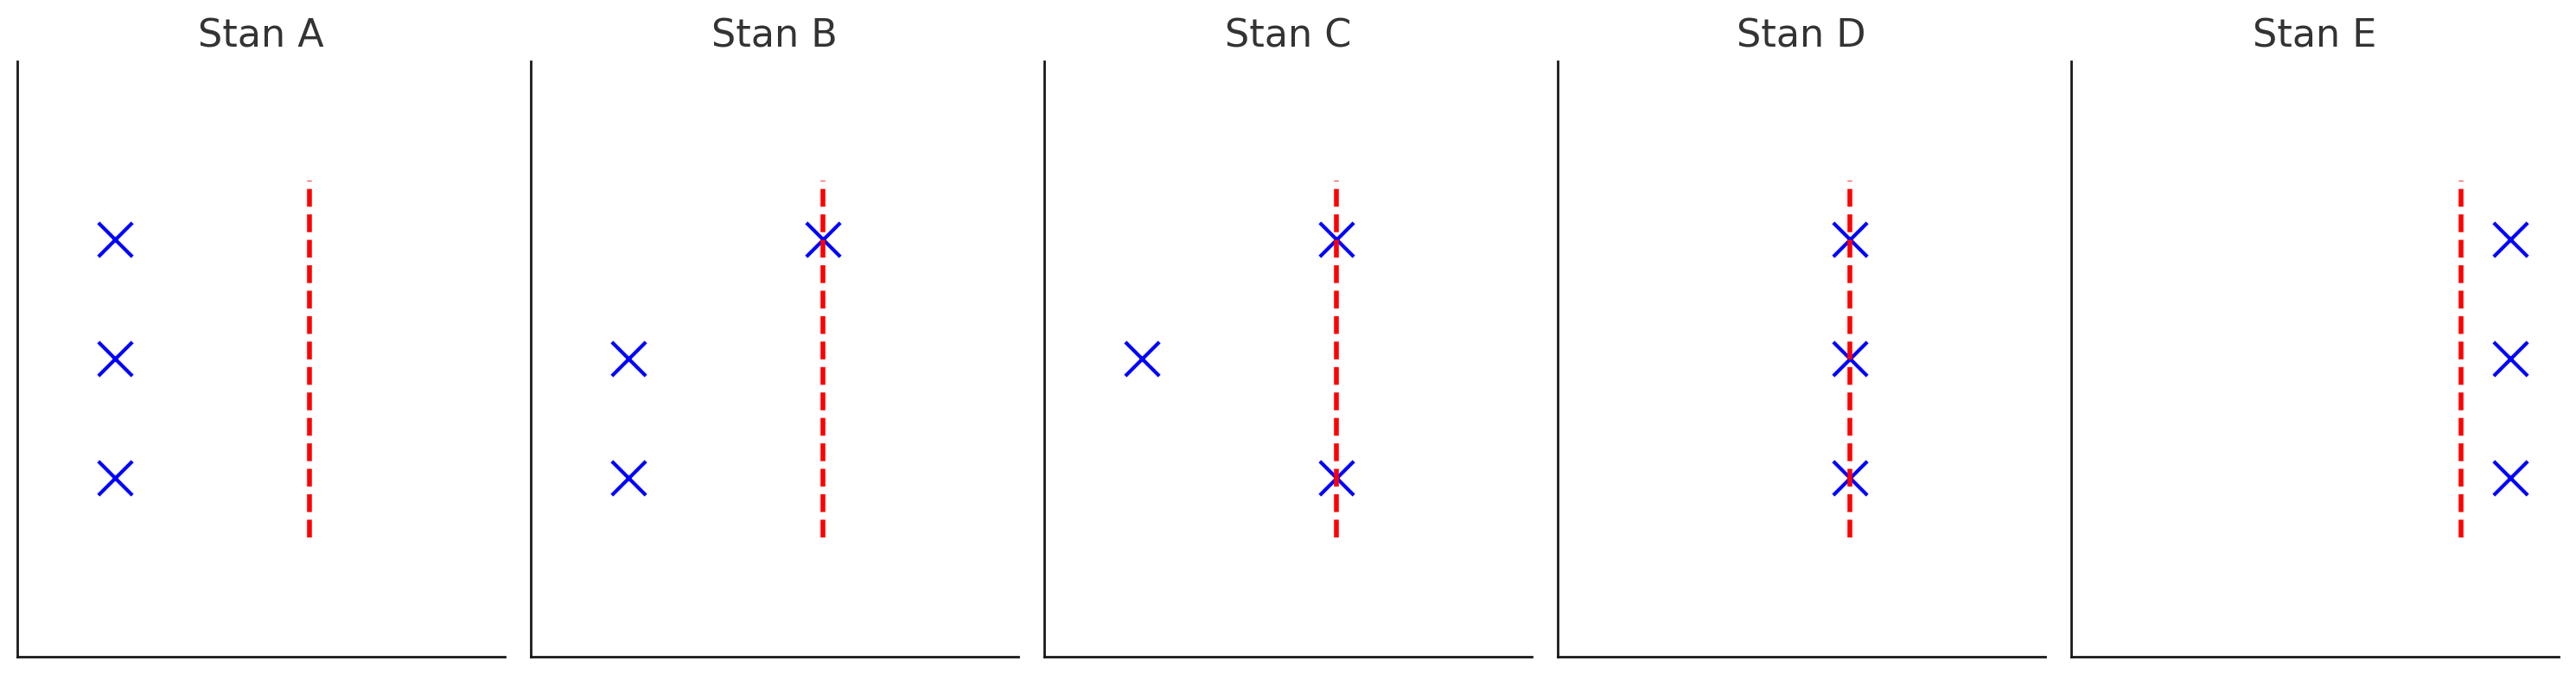
\includegraphics[width=\textwidth]{img/bariera.png}
\end{figure}

\subsection{Procesy działające na pierwszym planie, w tle i niezależne od terminala}
\begin{itemize}
    \item \texttt{jobs} - wyświetla listę procesów działających w tle
    \item \texttt{fg} - wznawia proces w pierwszym planie
    \item \texttt{bg} - wznawia proces pozostawiając go w tle
\end{itemize}
Przykładowe wyjście polecenia \texttt{jobs}
\begin{table}[ht]
\centering
\begin{tabular}{c c c}
    \texttt{[1]} & \texttt{Stopped} & \texttt{vim zad1.py} \\
    \texttt{[2]-} & \texttt{Running} & \texttt{ls -l} \\
    \texttt{[3]+} & \texttt{Stopped} & \texttt{python zad2.py} \\
\end{tabular}
\end{table}

Wyświetlany jest numer zadania oraz informacja, czy zadanie jest aktywne, czy czekające. Poprzez + oznaczone jest ostatnio uruchomione zadanie, natomiast - oznacza przedostatnie zadanie.

Przykład wznawiania poleceń:
\begin{itemize}
    \item \texttt{fg} 2 wznawia, na pierwszym planie, zadanie o numerze 2. 
    \item \texttt{bg} wznawia, w tle, ostatnio wykonane zadanie.
\end{itemize}

\texttt{nohup} - uruchamia proces, który nie jest zależny od terminala
\begin{itemize}
    \item\texttt{nohup ./skrypt.sh \&} - uruchamia proces w tle, który nie jest zależny od terminala. Proces nie jest zatrzymywany, gdy otrzyma sygnał SIGHUP.
\end{itemize}

\newpage \subsection{Elementy identyfikujące procesy}
\begin{itemize}
    \item\texttt{kill} - wysyła sygnał do procesu o podanym PID
    \item\texttt{killall} - wysyła sygnał do procesów o podanej nazwie 
    \item\texttt{pkill} - wysyła sygnał do procesów, których nazwa pasuje do podanego wzorca
    \item\texttt{pgrep} - wyświetla PID procesów, których nazwa pasuje do podanego wzorca
    \item\texttt{kill 1234} - wysyła (domyślny) sygnał SIGTERM do procesu o PID 1234
    \item\texttt{kill -s SIGKILL 1234} - wysyła sygnał SIGKILL do procesu o PID 1234
    \item \texttt{kill -s 9 1234} - wysyła sygnał SIGKILL do procesu o PID 1234
    \item\texttt{killall -s SIGKILL vim} - wysyła sygnał SIGKILL do procesów o nazwie vim
\end{itemize}

\textbf{Priorytet} określa jak często proces otrzymuje dostęp do zasobów. Priorytety w Unix/Linux zazwyczaj mogą przyjąć wartości od -20 do 19 (domyślnie proces ma priorytet 0). Niższe wartości oznaczają wyższy priorytet, czyli -20 to najwyższy priorytet, 19 to najniższy priorytet. Im niższy priorytet (większa liczba) tym proces posiada mniej czasu procesora.
\begin{itemize}
    \item\texttt{nice} -  pozwala na uruchomienie procesu z określonym priorytetem
    \item \texttt{renice} - pozwala na zmianę priorytetu procesu
    \item \texttt{nice -n 10 ./skrypt.sh} - uruchamia proces z priorytetem 10
    \item \texttt{renice -n 15 -p 1234} - zmienia priorytet procesu o PID 1234 na 15
\end{itemize}

Inne przydatne komendy:
\begin{itemize}
    \item \texttt{ps} - wyświetla listę aktualnie uruchomionych procesów, do których użytkownik ma dostęp
    \item \texttt{ps -L} - wyświetla informacje o wątkach
    \item \texttt{ps -f} - wyświetla informacje odnośnie listingu, tj. numer PPID czy liczba wątków w polaczeniu z \texttt{-L}
    \item \texttt{ps -e} - wyświetla wszystkie procesy systemowe
    \item \texttt{pstree} - wyświetla drzewo procesów
    \item \texttt{pstree -p} - wyświetla PID procesów
    \item \texttt{pstree -t} - wyświetla pełne nazwy wątków
    \item \texttt{exit} - powoduje zakończenie działania procesu i przekazuje jego kod wyjścia, który jest liczba jednobajtowa
    \item \texttt{return} - zwraca wartość funkcji, która jest liczba jednobajtowa
    \item \texttt{wait} - powoduje, że proces nadrzędny czeka na zakończenie procesu potomnego
    \item \texttt{trap} - przechwytuje sygnał i określa polecenia, które mają być wykonane po otrzymaniu sygnału
    \item \texttt{trap -l} - wyświetla listę sygnałów i ich identyfikatorów
    \item \texttt{trap -p} - wyświetla polecenia, jakie mają być wykonane po otrzymaniu sygnału
    \item \texttt{top, atop, htop, btop, glances} - interaktywne narzędzia do monitorowania procesów
\end{itemize}

\section{Zarządzanie zasobami}

\subsection{Szeregowanie procesów}
Jeżeli w komputerze wykorzystywana jest wielozadaniowość, często procesy lub wątki znajdujące się w tym samym stanie rywalizują o procesor.

\textbf{Program szeregujący} (ang. scheduler) to część systemu, która dokonuje wyboru procesu, który jako następny uzyska dostęp do procesora. Program szeregujący odpowiada również za wydajne działanie procesora podczas przełączania procesów.

W systemach operacyjnych można spotkać kilka \textbf{algorytmów szeregowania procesów}. Ich dwa główne typy to:
\begin{itemize}
    \item \textbf{Algorytmy szeregowania bez wywłaszczania} - proces może być zakończony jedynie przez zablokowanie lub zakończenie działania.
    \item \textbf{Algorytmy szeregowania z wywłaszczaniem} - scheduler może zatrzymać proces po określonym czasie, przed zakończeniem wykonania zadania i przydziela procesor innemu procesowi.
\end{itemize}

Schemat przełączania procesów:
\begin{enumerate}
    \item Przełączenie się z trybu użytkownika na tryb jądra;
    \item Papisanie stanu bieżącego procesu, i ewentualnie mapę pamięci, tak by można było ponownie uruchomić proces;
    \item Wybór nowego procesu na podstawie algorytmu szeregującego i załadowanie modułu z mapy pamięci; 
    \item Uruchomienie innego procesu.
\end{enumerate}

Kiedy należy wykonać szeregowanie?
\begin{itemize}
    \item Podczas tworzenia nowego procesu; scheduler musi zdecydować kiedy ma zostać uruchomiony.
    \item Podczas zakończenia pracy procesu; scheduler musi jaki proces ma go zastąpić.
    \item Podczas blokowania procesu przez semafor.
    \item Kiedy proces jest gotowy do wykonania działania.
    \item Kiedy wystąpi przerwanie.
\end{itemize}

Procesy można podzielić na dwa główne rodzaje ze względu na ich zadania i charakterystykę pracy:
\begin{itemize}
    \item Procesy \textbf{zorientowane na obliczenia} (ang. CPU-bound) to procesy, które przez większość czasu wykonują obliczenia.
    \item Procesy \textbf{zorientowane na wejście-wyjście} (ang. I/O-bound) to procesy, które przez większość czasu oczekują na zakończenie operacji wejścia-wyjścia
\end{itemize}

\subsection{Algorytmy szeregowania}
Algorytmy szeregowania są rożne w zależności od specyfiki środowiska, ponieważ rożne systemy realizują rożne zadania.

Przykładowe cele algorytmów szeregowania:
\begin{itemize}
    \item \textbf{Wszystkie systemy} - sprawiedliwe przydzielenie czasu procesora dla każdego procesu, sprawdzanie czy procesy przestrzegają zasad itp.
    \item \textbf{Systemy wsadowe} - maksymalizacja liczby wykonywanych zadań, zapewnienie ciągłości pracy procesora, minimalizacja czasu pomiędzy przetwarzaniem zadań, a jego zakończeniem. \textbf{Wywłaszczanie nie jest stosowane, albo jest stosowane z bardzo długim przydziałem czasowym dla procesora}.
    \item \textbf{Systemy interaktywne} - szybka odpowiedź na żądanie, proporcjonalne spełnianie oczekiwań użytkowników. \textbf{Wywłaszczanie pełni ważną rolę}, aby proces w nieskończoność nie korzystał z zasobów procesora (np. z powodu błędu w programie).
    \item \textbf{Systemy czasu rzeczywistego} - dotrzymywanie terminów, unikanie utraty danych. \textbf{Wywłaszczanie nie zawsze jest potrzebne}, ponieważ procesy po zakończeniu zadania szybko się blokują.
\end{itemize}

\subsection*{Szeregowanie w systemach wsadowych}
\textbf{Pierwszy zgłoszony, pierwszy obsłużony} (ang. first come, first served) polega na tym, że procesy otrzymują dostęp do procesora w kolejności w której zażądały do niego dostępu.

Przykładowe zalety algorytmu:
\begin{itemize}
    \item \textbf{łatwy do zrozumienia i zaimplementowania} (nie wykonuje skomplikowanych obliczeń);
    \item \textbf{Procesy są traktowane tak samo}, co może być korzystne w sytuacji, gdy mamy procesy o mniej więcej równym priorytecie.
\end{itemize}

Przykładowe wady algorytmu:
\begin{itemize}
    \item \textbf{Może doprowadzić do marnowania czasu} jeśli pierwszy proces w kolejce będzie trwał znacznie dłużej niż procesy, które będą później;
    \item \textbf{Nie dostosowuje się do wymagań} tj. priorytety, czy czas wykonania.
\end{itemize}

\textbf{Najkrótsze zadania najpierw obsłużone} (ang. shortest job first lub shortest job next) polega na tym, że program szeregujący wybiera proces o najkrótszym czasie działania.

Przykładowe zalety algorytmu:
\begin{itemize}
    \item \textbf{Algorytm minimalizuje średni czas przetwarzania wszystkich procesów}. Przykładowo dla zadań, które działają o czasach kolejno 8, 4, 2 minuty. przetwarzanie kolejnych zadań zajmie niecałe 12 min. ((8+12+14)/3);Początkowe przetwarzanie najkrótszych zadań zajmie niecałe 8 min. ((2+6+14)/3).
\end{itemize}

Przykładowe wady algorytmu:
\begin{itemize}
    \item \textbf{Konieczna jest znajomość czasów lub szacunkowych czasów wykonania zadań} co może być trudne do uzyskania w niektórych środowiskach;
    \item \textbf{Wszystkie zadania muszą być dostępne jednocześnie}, aby algorytm działał optymalnie.
\end{itemize}

\subsection*{Szeregowanie w systemach interaktywnych}
\textbf{Szeregowanie cykliczne} (ang. round robin) polega na tym, że każdemu procesowi przydzielany jest stały czas (kwant) w którym może wykonywać swoje działanie. Jeżeli proces nie zakończył swojego zadania po upływie czasu, zostaje on wywłaszczony i czeka na ponowny przydział do wykonania zadania. Jeżeli proces zakończył lub zatrzymał działanie, procesor przełącza kolejne zadanie.

Przykładowe zalety algorytmu:
\begin{itemize}
    \item \textbf{łatwy do zrozumienia i zaimplementowania};
    \item \textbf{procesy otrzymują taką samą szansę na dostęp do procesora}, co może być korzystne w sytuacji, gdy mamy procesy o mniej więcej równym priorytecie;
    \item \textbf{znany czas opóźnienia}, tzn. procesy wiedzą kiedy otrzymają ponownie dostęp.
\end{itemize}

Przykładowe wady algorytmu:
\begin{itemize}
    \item \textbf{wydłużony czas wykonywania procesów}, które mają długi czas działania;
    \item \textbf{niska efektywność podczas wykonywania zadań o różnym czasie działania} (czasami krótkotrwałe zadania muszą czekać, aż długotrwałe zadania wykonają swoje czynności);
    \item \textbf{nie dostosowuje się do obciążenia systemu}, ani do parametrów procesów tj. priorytety.
\end{itemize}

\textbf{Szeregowanie według priorytetów} (ang. priority scheduling) polega na tym, że każdemu procesowi jest przydzielany priorytet i program szeregujący wybiera proces o najwyższy priorytecie.

Przykładowe zalety algorytmu:
\begin{itemize}
    \item \textbf{dostosowanie szeregowania do charakterystyki zadania}, poprzez możliwość ustawienia różnych priorytetów;
    \item \textbf{pozwala na dynamiczne dostosowywanie priorytetów procesów w trakcie działania systemu}.
\end{itemize}

Przykładowe wady algorytmu:
\begin{itemize}
    \item \textbf{procesy o niższych priorytetach mogą być blokowane przez procesy o wyższych priorytetach};
    \item \textbf{właściwe określenie priorytetów dla różnych zadań czasami jest trudne};
    \item \textbf{może dojść do ”zapętlenia”, jeżeli dochodzi do stałej zmiany priorytetów}.
\end{itemize}

\textbf{Szeregowanie z wykorzystaniem kolejki priorytetów} (ang. multilevel queue scheduling) polega na podzieleniu procesów na różne poziomy priorytetów, przy czym procesy mogą zmieniać swoje położenie w zależności od wykonanych działań.

Zasada działania kolejki priorytetów:
\begin{itemize}
    \item Procesy należące do klasy o najwyższym priorytecie działają przez jeden kwant.
    \item Procesy należące do kolejnej klasy w hierarchii działają przez dwa kwanty.
    \item Procesy należące do kolejnej klasy w hierarchii działają przez cztery kwanty.
    \item Procesy należące do kolejnej klasy w hierarchii działają przez osiem kwantów itd.
    \item Jeżeli proces wykorzysta wszystkie swoje kwanty dostępne w danej klasie, jest przenoszony do klasy o niższym priorytecie.
\end{itemize}

Przykładowe zalety algorytmu:
\begin{itemize}
    \item \textbf{automatyczne dostosowanie priorytetów i kwantów czasu do rodzaju zadania} (krótkotrwałe zadania są wykonywane szybciej, a długotrwałe przenoszone do klas o niższym priorytecie).
\end{itemize}

Przykładowe wady algorytmu:
\begin{itemize}
    \item \textbf{bardziej skomplikowana implementacja};
    \item różne implementacji mogą działać różnie w zależności od ustawień kolejki priorytetów (\textbf{brak jednoznacznych reguł}).
\end{itemize}

\textbf{Szeregowanie gwarantowane} (ang. guaranteed scheduling) polega na zapewnieniu, że każdy proces otrzyma minimalny czas działania np. każdy z n użytkowników otrzyma 1/n mocy procesora.

Przykładowe zalety algorytmu:
\begin{itemize}
    \item zapewnienie, że \textbf{określone zadania zostaną wykonane w określonym czasie};
    \item \textbf{procesy mogą być obsługiwane zgodnie z wymaganiami sprzętowymi}.
\end{itemize}

Przykładowe wady algorytmu:
\begin{itemize}
    \item \textbf{możliwe marnowanie zasobów procesora}, gdy nie są wykorzystywane wszystkie;
    \item \textbf{przeciążenie systemu w przypadku dużej liczby procesów}; 
    \item \textbf{wymagana jest precyzyjna ocena czasu wykonania zadań}.
\end{itemize}

\textbf{Szeregowanie loteryjne} (ang. lottery scheduling) polega na tym, że każdy proces otrzymuje tzw. bilety, następnie program szeregujący wykonuje ”losowanie” biletu, który otrzyma dostęp do procesora (im więcej biletów ma proces tym większa szansa, że zostanie wybrany).

Przykładowe zalety algorytmu:
\begin{itemize}
    \item \textbf{procesy, które mają mało biletów, nadal mają szansę na dostęp do zasobów procesora co oznacza, że nie zostaną zablokowane};
    \item \textbf{procesy mogą dynamicznie zmieniać liczbę swoich biletów w trakcie działania systemu}.
\end{itemize}

Przykładowe wady algorytmu:
\begin{itemize}
    \item \textbf{przydzielenie właściwej liczby biletów może być trudne};
    \item \textbf{losowanie wprowadza dodatkowe obliczenia}, które mogą powodować opóźnienie wykonywanego zadania.
\end{itemize}

Algorytmy szeregowania mogą mieć przypisane wagi dla użytkowników,
którzy uruchamiają procesy.

Przykład:
Załóżmy, że z systemu, który wykorzystuje algorytm cykliczny, korzysta dwóch użytkowników. 
\begin{itemize}
    \item Pierwszy użytkownik uruchomił cztery procesy (P1P2P3P4), drugi uruchomił jeden proces (P5). 
    \item Jeżeli każdy użytkownik ma 50\% czasu procesora: możliwa kolejność wykonywania procesów: P1P5P2P5P3P5P4P5P1P5P2P5... 
    \item Jeżeli pierwszy użytkownik ma dwa razy więcej czasu procesora niż drugi: możliwa kolejność wykonywania procesów: P1P2P5P3P4P5P1P2P5P3P4P5...
\end{itemize}

\subsection{Zakleszczenie}
\textbf{Zakleszczenie} (ang. deadlock) to sytuacja w której dochodzi zablokowania pewnego zbioru procesów, np. procesy oczekują na pewien zasób, który jest zajmowany przez inne procesy.

Zasobem może być urządzenie sprzętowe, blok informacji itp.
Rodzaje zasobów:
\begin{itemize}
\item \textbf{zasoby z możliwością wywłaszczania}, to zasoby, które można odebrać procesom bez skutków ubocznych, np. pamięć;
\item \textbf{zasoby bez możliwości wywłaszczania}, to zasoby, których nie można odebrać procesom bez skutków ubocznych, np. wypalana płyta CD
\end{itemize}

Warunki powstania zakleszczenia zasobów. Wszystkie warunki muszą być spełnione by doszło do zakleszczenia.
\begin{itemize}
    \item \textbf{wzajemne wykluczanie} - każdy zasób jest przypisany do jednego procesu, albo jest dostępny;
    \item \textbf{procesy, które mają przydzielony zasób, żądają nowych zasobów};
    \item \textbf{zasoby przydzielone wcześniej nie mogą być odebrane siłą};
    \item \textbf musi istnieć cykl, składający się z co najmniej dwóch procesów, w których \textbf{każdy proces oczekuje na zasób, który jest kontrolowany} przez następny proces w cyklu.
\end{itemize}

\subsection{Przykładowe sposoby postępowania}
\subsection*{Przykładowy algorytm ignorowania zakleszczeń}
\textbf{Algorytm strusia} polega na tym, że ”wkładamy głowę w piasek” i udajemy, że problemu nie ma.

\subsection*{Przykładowe algorytmy wykrywania zakleszczeń}
Przykładowy \textbf{algorytm działający dla zasobów jednego typu}, np. dla systemu posiadającego jedną drukarkę, jedną nagrywarkę itd. Schemat działania:
\begin{enumerate}
    \item Początkowo tworzymy graf procesów i zasobów.
    \item Tworzymy pustą listę i umieszczamy ”losowo” wybrany wierzchołek grafu.
    \item Następnie umieszczamy losowo wybrany \textbf{wierzchołek, który ma łuk wychodzący z naszego wierzchołka}
    \item Jeżeli nie istnieje żaden łuk wychodzący \textbf{usuwamy ostatnio wybrany wierzchołek} i sprawdzamy czy możemy wybrać dla niego łuk.
    \item Jeżeli lista jest pusta, \textbf{sprawdzamy czy istnieje inny wierzchołek od którego wcześniej nie zaczynaliśmy}, jeżeli, tak, \textbf{umieszczamy go w liście}, w przeciwnym razie kończymy działanie wiedząc, że \textbf{nie ma zakleszczeń}.
    \item Podczas umieszczania wierzchołka w liście sprawdzamy, czy nie został on już wcześniej umieszczony. Jeżeli tak, wiemy, że \textbf{graf posiada cykl i występuje zakleszczenie}.
\end{enumerate}

Przykładowy \textbf{algorytm działający dla wielu zasobów każdego typu}.
\begin{enumerate}
    \item Tworzymy dwa wektory określające istniejące ($V_E$) i dostępne zasoby ($V_A$) oraz dwa macierze określające przydział ($M_C$) i zapotrzebowanie ($M_R$) zasobów dla procesów.
    \item Wybieramy wcześniej niewybrany proces, którego wiersz macierzy $M_R$ jest mniejszy lub równy niż wektor $V_A$.
    \item Jeżeli taki proces nie istnieje kończymy działanie z informacją, że \textbf{niewybrane procesy są zakleszczone}. Jeżeli zostaną wybrane wszystkie procesy \textbf{kończymy działanie z informacją, że zakleszczenia nie występują}.
    \item Jeżeli wybierzemy proces dodajemy do $V_A$ odpowiedni wiesz z $M_C$.
\end{enumerate}

\subsection*{Przykładowe sposoby usuwania wykrytych zakleszczeń}
Jeżeli zakleszczenie zostanie wykryte, algorytmy podejmują działania mające na celu usunięcie zakleszczenia.
\begin{itemize}
    \item \textbf{Kończenie pracy procesów poprzez wysłanie sygnału} - można zakończyć pracę jednego lub więcej procesów, które są zakleszczone lub procesu, który nie jest zakleszczony, by zwolnić zasoby.
    \item \textbf{Cofanie operacji} - stan procesu jest rejestrowany (stan procesu jest zapisywany do pliku) i w przypadku powstania zakleszczenia można cofnąć proces do poprzedniego stanu.
    \item \textbf{Wywłaszczanie procesów} - zakleszczony proces można wywłaszczyć, dzięki czemu zwolni zasoby
\end{itemize}

\subsection{Sposoby unikania zakleszczeń zasobów}
\textbf{Algorytm bankiera} polega na sekwencyjnym przyznawaniu procesom zasobów w taki sposób, aby nie dopuścić do sytuacji, w której jakiś proces nie będzie w stanie zakończyć swojego działania. Algorytm bankiera może nie działać efektywnie, ponieważ procesy nie zawsze wiedzą z góry jakie zasoby są im potrzebne i wymaga informacji na temat przyszłych żądań
Schemat działania algorytmu bankiera:
\begin{itemize}
    \item \textbf{Wybieramy proces, który spełnia warunek} - proces, który nie został zakończony i dla którego potrzebne zasoby są mniejsze niż zasoby dostępne.
    \item \textbf{Przydzielamy zasoby procesowi} - jeżeli proces spełnia warunek, przydzielamy zasoby i oznaczamy proces jako zakończony.
    \item \textbf{Zwalniamy zasoby} - jeżeli proces zakończył działanie i zwalniamy zasoby.
    \item \textbf{Kończymy działanie} - jeżeli wszystkie procesy zostały zakończone, kończymy działanie.
\end{itemize}

Unikanie zakleszczeń w obecnych systemach polega na usunięciu jednego z czterech warunków, który powoduje powstanie zakleszczenia:
\begin{itemize}
    \item wzajemne wykluczanie - \textbf{umożliwienie na dostęp do zasobu przez wiele procesów}.
    \item przydzielenie i oczekiwanie zasobu - \textbf{ustalenie z góry, jakie zasoby są potrzebne} (wówczas można zastosować algorytm bankiera).
    \item brak możliwości odebrania zasobu - \textbf{możliwość odebrania zasobów procesowi (np. wywłaszczanie)}.
    \item cykl składający się z dwóch procesów - \textbf{wprowadzenie reguł, które sprawią, że proces zwolni zasób jeśli potrzebuje kolejnego}.
\end{itemize}

\subsection{Inne problemy}
\begin{itemize}
    \item \textbf{Zakleszczenie komunikacyjne} to sytuacja w której dwa lub więcej procesów czeka na odpowiedź od siebie nawzajem. Rozwiązaniem problemu może być ustawienie limitu czasu (ang. timeout).
    \item \textbf{Uwięzienie} (ang. livelock) to sytuacja, w której co najmniej dwa procesy lub wątki, wykonują swoje zadania w taki sposób, że blokują się one nawzajem, co może uniemożliwić dokończenie zadania. Przykładowo, kiedy jeden wątek oczekuje na odpowiedź od drugiego, podczas gdy drugi wątek wykonuje obliczenia w nieskończonej pętli: w tej sytuacji wątki wzajemnie się blokują.
    \item \textbf{Zagłodzenie} (ang. starvation) to sytuacja, w której proces lub wątek, nie może otrzymać dostatecznie dużej liczby zasobów, by kontynuować swoje działanie, co w konsekwencji może doprowadzić do zakleszczenia lub opóźnienia. Przykładowo z zagłodzeniem mamy do czynienia, kiedy algorytm szeregowania wybiera najkrótsze zadania i krótkich zadań jest na tyle dużo, że długie zadania będą w nieskończoność odwlekane.
\end{itemize}

\section{Zagrożenia i bezpieczeństwo}
\subsection{Rodzaje ataków}
\begin{itemize}
    \item \textbf{Tylne drzwi} (ang. backdoor) to technika polegająca na zaprojektowaniu oprogramowania lub systemu, w taki sposób, że możliwy jest dostęp do zasobów z pominięciem mechanizmów zabezpieczających tj. uwierzytelnianie. Jedynym skutecznym sposobem na zabezpieczenia, przed wprowadzeniem tylnych drzwi, są regularne przeglądy kodu, przez zespół programistów pracujący nad projektem.
    \item \textbf{Fałszywe logowanie} (ang. login spoofing) to technika, która ma na celu kradzież danych logowania, polegająca na podszywaniu się pod prawidłowe miejsce logowania. Jedynym skutecznym sposobem na zapobieganie takim działaniom, jest uruchamianie możliwości logowania przez kombinację klawiszy, która jest obsługiwana przez system operacyjny, a nie przez program użytkownika. 
    \item \textbf{Fałszywy adres IP} (ang. IP spoofing) to technika, polegająca na fałszowaniu adresu IP, aby ukryć tożsamość w celu uzyskania dostępu. Przykładowe sposoby zapobiegania:
\begin{itemize}
    \item \textbf{filtracja ruchu} - odrzucanie pakietów, które nie pochodzą z zaufanego źródła;
    \item \textbf{uwierzytelnianie} - sprawdzanie tożsamości użytkownika;
    \item \textbf{monitorowanie ruchu sieciowego} - sprawdzanie, czy nie występuje podejrzany ruch sieciowy.
    \item \textbf{firewall} - zapobieganie dostępowi do zasobów sieciowych.
    \item \textbf{Stosowanie silnych haseł} - zabezpieczenie przed atakami typu brute force.
\end{itemize}
    \item \textbf{Uniemożliwienie dostępu} (ang. denial of service, skr. DoS) atak mający na celu uniemożliwienie lub utrudnienie dostępu do zasobów poprzez przepełnienie ich ruchem sieciowym.
Popularne rodzaje ataków to:
\begin{itemize}
    \item \textbf{ping flood} - atak polegający na wysyłaniu dużej liczby pakietów ICMP
    \item \textbf{SYN flood} - atak polegający na generowaniu dużej liczby połączeń TCP, co powoduje przepełnienie kolejki połączeń
    \item \textbf{HTTP flood} - atak polegający na generowaniu dużej liczby zapytań HTTP
\end{itemize}
    Popularnym rodzajem ataku DoS jest \textbf{rozproszone uniemożliwienie dostępu} (ang. distributed denial of service, skr. DDoS), który jest przeprowadzany z wielu komputerów (np. zombie).
    \item \textbf{Atak pośrednika} (ang. man in the middle, skr. MitM) atak polegający na umiejscowieniu cyberprzestępcy pomiędzy dwiema stronami komunikującymi się w celu przechwycenia lub modyfikacji przesyłanej wiadomości. Popularne rodzaje ataków:
\begin{itemize}
    \item modyfikacja tablicy ARP, która przechowuje powiązania adresów IP z adresemMAC urządzeń w sieci lokalnej (ang. ARP spoofing);
    \item modyfikacja konfiguracji DNS, tak aby przekierowywał żądanie na inny adres IP (ang. DNS spoofing);
    \item zmuszenie użytkownika do korzystania z niezabezpieczonej strony, która kiedyś była zabezpieczona protokołem SSL/TLS (HTTPS), w taki sposób, że żądania początkowo będą wysyłane do pośrednika, zanim zostaną wysłane do właściwego serwera (ang. SSL strip); 
    \item stworzenie fałszywego WiFi, które nadsłuchuje ruch.
\end{itemize}
\end{itemize}

\subsection{Wykorzystanie błędów w kodzie}
\textbf{Exploit} to program lub technika wykorzystująca błędy w oprogramowaniu w celu wykonania szkodliwej czynności.

\textbf{Zero-day exploit} wykorzystuje błędy w kodzie, które nie są znane dla twórców oprogramowania.

Przykładowe szkody, jakie mogą wyrządzić exploity:
\begin{itemize}
    \item otwieranie tylnych drzwi, w celu przejęcia kontroli nad komputerem;
    \item kradzież danych użytkownika;
    \item utrudnienie pracy z systemem operacyjnym;
    \item rozprzestrzenianie złośliwego oprogramowanie.
\end{itemize}

\textbf{Atak z wykorzystaniem przepełnienia bufora} to nadpisanie kolejnych komórek pamięci, które nie zostały zaalokowane do wykorzystania np. tablicy oraz mogą nadpisać obszar pamięci, który jest używany przez system operacyjny.
\subsection{Złośliwe oprogramowanie}
\textbf{Złośliwe oprogramowanie} (ang. malware) to oprogramowanie, celem jest powodowanie szkód.
\begin{itemize}
    \item \textbf{Zombie} to komputer, który jest zdalnie kontrolowany przez cyberprzestępce.
    \item \textbf{Botnet} biór komputerów zombie.
    \item \textbf{Wirus} to rodzaj złośliwego oprogramowania, które są zdolne do reprodukcji poprzez dołączenie swojego kodu do innych programów lub systemów. Po napisaniu wirusa, autor może użyć do wstrzyknięcia go do pliku poprzez narzędzie tj. \textbf{dropper}.
    \item \textbf{Robak} to rodzaj złośliwego oprogramowania, które są zdolne do reprodukcji poprzez wykorzystanie błędów i niedopatrzeń w innych oprogramowaniach.
    \item \textbf{Koń} trojański to rodzaj złośliwego oprogramowania, które podszywa się pod pozornie nieszkodliwe oprogramowanie, które jest instalowane świadomie przez użytkownika.
    \item \textbf{Bomba logiczna} to rodzaj złośliwego oprogramowania, które jest uruchamiany po wykonaniu określonej czynności, np. po zalogowaniu się użytkownika, czy po uruchomienie programu. Bomby logiczne mogą być potajemnie tworzone przez programistów (np. w ramach ewentualnej zemsty za zwolnienie z pracy). Można wykorzystać wirusy, robaki, konie trojańskie do umieszczania bomblogicznych.
    \item \textbf{Rootkit to rodzaj złośliwego oprogramowania}, którego celem jest ukrywanie istnienia złośliwych oprogramowań przed użytkownikiem lub wykonywania szkodliwych działań na zainfekowanym komputerze. Przykładowe miejsca ukrywania rootkitów to: przestrzenie jądra systemu operacyjnego, sterowniki urządzeń, biblioteki systemowe, rejestry systemowe, aplikacje, pamięć, warstwa wizualizacji.
    \item \textbf{Oprogramowanie szpiegujące} (ang. spyware) to rodzaj złośliwego oprogramowania, które gromadzi dane na temat aktywności użytkownika na komputerze i przesyła zgromadzone informacje.
    \item \textbf{Rejestrator klawiatury} (ang. keylogger) to rodzaj złośliwego oprogramowania, które rejestruje aktywność na klawiaturze użytkownika, oraz wysyła informację na temat wciśniętych klawiszy.
    \item \textbf{Oprogramowanie żądające okupu} (ang. ransomware) to rodzaj złośliwego oprogramowania, które blokuje dostęp do danych znajdujących się na komputerze, a następnie wyświetla informację na temat żądania okupu w zamian za odblokowanie danych.
\end{itemize}
\subsection{Zapora sieciowa}
\textbf{Zapora sieciowa} (ang. firewall) to oprogramowanie lub urządzenie, które służy do blokowania niepowołanego dostępu do komputera lub sieci wewnętrznej, przez sieć zewnętrzną, poprzez monitoring i kontrolę ruchu sieciowego. Przykładowe rodzaje zapór sieciowych:
\begin{itemize}
    \item \textbf{zapora sieciowa stanowa} (ang. stateful firewall) to rodzaj zapory sieciowej, która analizuje bieżący stan połączeń sieciowych, dzięki czemu skuteczniej sobie radzą z niektórymi rodzajami ataków tj. ataki polegające na ustawianiu połączeń. 
    \item \textbf{zapora sieciowa osobista} (ang. personal firewall) to rodzaj zapory sieciowej, będąca oprogramowaniem, która chroni urządzenie (np. komputer), poprzez monitoring ruchu wychodzącego i przychodzącego oraz kontrolę aplikacji mających dostęp do sieci.
    \item \textbf{zapora sieciowa aplikacji} (ang. application firewall) to rodzaj zapory sieciowej, która analizuje protokoły działające na poziomie aplikacji sieciowej, np. może odpowiadać za kontrolę ruchu sieciowego na poziomie protokołu tj. HTTP, TCP, FTP. 
    \item zapora sieciowa posiadająca zaimplementowany \textbf{system wykrywania i zapobiegania włamań} (ang. intrusion detection system, intrusion prevention system, skr. IDS/IPS), może nie tylko kontrolować nagłówki pakietów, ale też wykrywać i zapobiegać atakom sieciowym.
\end{itemize}
\subsection{Programy zwalczające złośliwe oprogramowanie}
\textbf{Program zwalczający złośliwe oprogramowanie} umożliwia zwalczenie złośliwego oprogramowania np. robaki, wirusy czy spyware.
\begin{itemize}
    \item \textbf{Skaner antywirusowy} polega na skanowaniu plików znajdujących się na dysku w celu poszukiwania zainfekowanych plików.
    \item \textbf{Weryfikatory integralności} (ang. integrity checking) to narzędzie, które na początku rozpoczyna skanowanie w poszukiwaniu wirusów i po nabraniu pewności o braku wirusów, wyznacza sumę kontrolną dla każdego pliku wykonywalnego. Podczas następnego skanowania sprawdzane jest, czy suma kontrolna jest taka sama.
    \item \textbf{Weryfikatory zachowań} (ang. behavioral checking) to narzędzie, które na na celu monitorowanie aktywności systemu w celu wykrycia podejrzanych działań.
\end{itemize}

\subsection{Inne mechanizy zabezpieczenia}
\begin{itemize}
    \item \textbf{Podpisywanie kodu} (ang. code signing) polega na stosowaniu podpisu cyfrowego do utworzonych produktów. Producent generuje klucz publiczny i prywatny oraz generuje kod, który jest zwracany przez funkcję skrótu, uruchomionej dla kodu programu. Producent podpisuje oprogramowanie kodem, poprzez zaszyfrowanie go kluczem prywatnym. Podpis jest przekazywany z oprogramowaniem. Kiedy użytkownik uruchamia program, uruchamiana jest funkcja skrótu, która zapisuje wynik. Mechanizm weryfikujący odszyfrowuje, przy pomocy klucza publicznego, podpis dołączony do oprogramowania. Jeżeli kod zwrócony przez funkcje skrótu i kod odszyfrowanego podpisu jest taki sam, to program jest akceptowalny, w przeciwnym razie jest uznawany za sfałszowany.
    \item \textbf{Wtrącanie do więzienia} (ang. jailing) to mechanizm, który polega na sprawdzeniu zachowania procesu i w razie potrzeby, izolowania im dostępu do zasobów systemowych. Nowy proces jest monitorowany przez zaufany proces systemowy, który decyduje czy żądane wywołanie systemowe może zostać zrealizowane. Oznacza to, że podejrzane zachowania można wykryć i wyeliminować zanim narobią szkód w systemie.
    \item \textbf{Izolowanie} (ang. sandboxing) to mechanizm, który polega na uruchamianiu zadań w odizolowanym kontrolowanym środowisku. Przestrzeń adresów wirtualnych jest podzielona na obszary o tej samej wielkości, które nazywamy piaskownicami (ang. sandboxes). Piaskownice zawierają mechanizmy, które uniemożliwiają możliwość wykonania skoku do innej piaskownicy oraz pobierania z niej danych itp.
    \item \textbf{Wykrywanie włamań} z użyciem modeli statycznych (ang. static modelbased intrusion detection) to mechanizm wykrywania włamań na podstawie modelu. Przykładowy modelem może być graf wywołań systemowych. Można zastosować jailing w którym proces monitorujący kończy zadanie, którego zachowanie jest niezgodne z modelem.
\end{itemize}

\section{Administrowanie}

\subsection{Rola użytkownika root w Linux}
\textbf{root} - Użytkownik o najwyższych uprawnieniach w systemie. może przeprowadzać wszelkie zadania administracyjne, dlatego czasami jest nazywany superużytkownikiem.
\begin{itemize}
    \item \texttt{su} - zmienia tożsamość użytkownika
    \item \texttt{sudo} - pozwala na wykonanie polecenia jako użytkownik root lub jako inny użytkownik (w zależności od konfiguracji)
    \item \texttt{sudo su} - uruchamia powłokę jako użytkownik root
\end{itemize}

\subsection{Zadania cykliczne}
\texttt{cron} - demon opowiedzialny za uruchomianie zadań wg określonego harmonogramu.
\begin{itemize}
    \item \texttt{crontab} - umożliwia zarządzanie poleceniami cyklicznymi cron
    \item \texttt{crontab -e} - otwiera edytor, umożliwiający zmianę zawartości pliku crontab
    \item \texttt{crontab -l} - wyświetla listę zaplanowanych zadań.
    \item \texttt{crontab -r} - usuwa plik crontab (usuwa zadania).
    \item \texttt{crontab -u} - lmielewczyk -l wyświetla listę zaplanowanych zadań użytkownika lmielewczyk.
\end{itemize}

Każdy wiersz pliku crontab zawiera komentarze poprzedzone znakiem \#, albo wiersz odpowiadający cyklicznemu poleceniu w formacie:

\texttt{minuta godzina dzień\_miesiąca miesiąc dzień\_tygodnia polecenie}

\subsection{Pliki}
\begin{itemize}
    \item \textbf{/etc/sudoers} - zawiera definicję uprawnień w stosunku do polecenia sudo w systemach Unix/Linux.
    \item \textbf{/etc/passwd} - zawiera listę użytkowników, którzy są rozpoznawani przez Linuxa. Podczas logowania system pobiera dane z pliku, aby określić m.in. UID, czy katalog domowy użytkownika.
    \item \textbf{/etc/group} - zawiera informację na temat grup, które są dostępne w systemie
    \item \textbf{/etc/shadow} - zawiera zaszyfrowane hasła i inne informacje odnośnie zarządzania hasłami. Plik jest chroniony przed programami do łamania haseł i może być odczytywany jedynie przez użytkownika root
\end{itemize}

\subsection{Polecenia}
\begin{itemize}
    \item \texttt{chfn} - zmienia informacje o użytkowniku.
    \item \texttt{chown} - zmienia właściciela i przynależność grupy plików i katalogów.
    \item \texttt{chage} - ustawia ważność hasła użytkownika.
    \item \texttt{chsh} - pozwala zmienić domyślną powłokę.
    \item \texttt{useradd} - dodaje nowe konto użytkownika.
    \item \texttt{usermod} - modyfikuje atrybuty konta użytkownika.
    \item \texttt{userdel} - usuwa konto użytkownika.
    \item \texttt{adduser} - dodaje nowego użytkownika.
    \item \texttt{deluser} - usuwa użytkownika.
    \item \texttt{groupadd, addgroup} - dodaje nową grupę.
    \item \texttt{groupdel, delgroup} - usuwa grupę.
    \item \texttt{groupmod} - modyfikuje atrybuty grupy.
\end{itemize}

\subsection{Moduł uwierzytelniania PAM}
Moduł uwierzytelniania \textbf{PAM} (ang. pluggable authentication modules) to modularny system umożliwiający kontrolę uwierzytelniania w systemach operacyjnych Unix/Linux. Pliki konfiguracyjne PAM znajdują się w katalogu \texttt{/etc/pam.d/}. Każda usługa ma własny plik konfiguracyjny, np. \texttt{/etc/pam.d/login, /etc/pam.d/passwd, /etc/pam.d/su}.

\subsection{Funkcja pojedynczego logowania}
\textbf{Funkcja pojedynczego logowania} (skr. SSO, ang. single sign-on) pozwala na uzyskanie dostępu do dowolnego systemu, usługi lub aplikacji, przy pomocy tego samego loginu i hasła. SSO zazwyczaj zawiera informacje tj. nazwa użytkownika, (zaszyfrowane) hasło, identyfikator użytkownika (UID), adres email.

Podstawowe elementy SSO:
\begin{enumerate}
    \item \textbf{Scentralizowany magazyn katalogów} - miejsce, gdzie przechowywane są informacje na temat użytkowników, takie jak dane uwierzytelniające, uprawnienia i atrybuty. Przykładowe scentralizowane magazyny katalogów:
    \begin{itemize}
        \item LDAP (ang. lightweight directory access protocol) (np. OpenLDAP)
        \item Active Directory
    \end{itemize}
    \item \textbf{Narzędzie do zarządzania danymi użytkowników} - narzędzie umożliwiające administrację użytkownikami, ich danymi i uprawnieniami. Przykładowe narzędzia do zarządzania danymi użytkowników
    \begin{itemize}
        \item Apache Directory Studio (dla LDAP)
        \item Active Directory Users and Computers (dla Active Directory)
    \end{itemize}
    \item \textbf{Mechanizm uwierzytelniania} - mechanizm uwierzytelniania potwierdzają tożsamość użytkownika na podstawie dostarczonych danych, tj. login i hasło. Przykładowe mechanizmy uwierzytelniania:
    \begin{itemize}
        \item Kerbersos (uwierzytelnianie oparte na biletach)
        \item SSSD (ang. system security services daemon) (demon pośredniczący między PAM a źródłami danych tj. LDAP, Active Directory)
        \item LDAP (bezposrednio)
    \end{itemize}
    \item \textbf{Scentralizowane funkcje sprawdzające atrybuty użytkownika} - funkcje odpowiadające za weryfikację atrybutów użytkownika, takich jak uprawnienia czy role. przykładowe scentralizowane funkcje sprawdzające atrybuty użytkownika:
    \begin{itemize}
        \item w systemach Unix/Linux plik /etc/nsswitch.conf zawiera konfiguracje źródeł danych
    \end{itemize}
    \item \textbf{Protokoły komunikacyjne} - protokoły służące do komunikacji między aplikacjami a serwerem uwierzytelniającym.
\end{enumerate}

\subsection{Rejestrowanie dzienników w Linux}
System \textbf{syslog} to narzędzie, którego celem jest tworzenie plików dziennika oraz daje możliwość konfiguracji rejestrowania zdarzeń. Większość plików dziennika systemu jest zazwyczaj przechowywane w katalogu \texttt{/var/log}. System syslog korzysta z konfiguracji znajdującej się w pliku \texttt{/etc/rsyslog.conf}. System syslog zarządzany jest przez demona \texttt{rsyslogd}, albo przez demona \texttt{syslogd}. Syslog umożliwia sortowanie komunikatów ze względu na ich źródło (usługi) i poziom ważności oraz kierowanie ich do różnych miejsc tj. pliki dzienników, pliki terminali, czy inne komputery. Przykładowe usługi systemu syslog: \texttt{authenctication, cron, daemon, kernel, mail, mark, syslog, user}.

System \textbf{systemd} to narzędzie służące do przechowywania plików dziennika. System systemd przechowuje dzienniki w plikach binarnych, w większości przypadków są przechowywane w folderze \texttt{/var/log/journald}. Systemd korzysta z konfiguracji znajdującej się w pliku: \texttt{/etc/systemd/journald.conf}, przy czym własne konfiguracje można wprowadzać do folderu: \texttt{/etc/systemd/journald.conf.d}.  System systemd zarządzany jest przez demona \texttt{systemd-journald}.

Systemy syslog i systemd to narzędzia, które są powszechnie stosowane. Oba systemy dostarczają istotne funkcje, które sprawiają, że mogą ze sobą współpracować (np. syslog może odbierać komunikat z różnych wtyczek wejściowych).

Inne narzędzia:
\begin{itemize}
    \item \textbf{logrotate} - umożliwia zarządzanie dziennikami w Linuxie (tj. automatyczne przenoszenie, usuwanie, kompresja)
    \item \textbf{ELK Stack} - połączenie narzędzi:
    \begin{itemize}
        \item \textbf{elasticsearch} - posiada funkcje przeszukiwania, analizy i przechowywa- nia dużej ilości danych,
        \item \textbf{logstash} - służy do przetwarzania, przekształcania i przesyłania logów z różnych źródeł do elasticsearch,
        \item \textbf{kibana} - dostarcza interfejs webowy do eksploracji, analizy i wizual- izacji danych przechowywanych w elasticsearch
    \end{itemize}
    (dobry wybór jeśli priorytetem jest wszechstronność tzn. obsługa różnych formatów).
    \item \textbf{Graylog} - posiada jeden główny serwer i opcjonalną bazę danych (dobry wybór jeśli priorytetem jest monitorowanie logów lub łatwa konfiguracja).
    \item \textbf{Apache Druid} - system bazodanowy, który służy do przetwarzania i analizy dużej ilości danych (dobry wybór jeśli priorytetem jest szybka analiza danych) 
\end{itemize}

\newpage \subsection{Narzędzia monitorujące}
\begin{itemize}
    \item \textbf{collectd} - umożliwia zbieranie danych odnośnie wydajności systemu. Narzędzie collectd tworzy demona collectd i korzysta z konfiguracji w pliku: \newline\texttt{/etc/collectd/collectd.conf}. Collectd zbiera różne dane dotyczące wydajności systemu, takie jak tj. zużycie CPU, obciążenie systemu, ilość dostępnej pamięci, statystyki dysków, informacje o sieci, temperatury itd. Dane te mogą posłużyć do generowania raportów, analizy i monitorowania systemu.
    \item \textbf{Nagios, Icinga} - popularne narzędzia monitorujące systemy, sieci, aplikacje itp. Narzędzia Nagios i Icinga posiadają interfejs WWW umożliwiające wygodne zarządzanie oraz mechanizmy umożliwiające tworzenie raportów i archiwizacji monitorowanych danych. Narzędzia Nagios i Icinga mogą powiadamiać administratorów o awariach i innych istotnych zdarzeniach za pomocą różnych kanałów tj. email, SMS itp. Nagios i Icinga mogą korzystać z danych zbieranych przez collectd, następnie przekazując je do narzędzi wizualizacji danych.
\end{itemize}

\subsection{journalctl i systemctl}
\begin{itemize}
    \item \texttt{journalctl} - przeszukuje i analizuje logi wygenerowane przez system systemd.
    \item \texttt{journalctl -u ssh} - wyświetla dzienniki wygenerowane przez ssh.
    \item \texttt{journalctl -n 100 -D /var/log/journal/2000/} - wyświetla ostatnie 100 wersów z dziennika w katalogu.
    \item \texttt{journalctl -since yesterday -until now} - wyświetla komunikaty od wczoraj do chwili obecnej.
    \item \texttt{systemctl} - umożliwia zarządzanie usługami systemowymi
    \item \texttt{sudo systemctl start mysql} - uruchomienie usługi mysql.
    \item \texttt{sudo systemctl stop mysql} - zatrzymanie usługi mysql.
    \item \texttt{sudo systemctl restart mysql} - restart usługi mysql.
    \item \texttt{sudo systemctl status mysql} - sprawdzenie statusu usługi mysql
    \item \texttt{sudo systemctl enable mysql} - włączenie usługi mysql przy starcie systemu.
    \item \texttt{sudo systemctl disable mysql} - wyłączenie usługi mysql przy starcie systemu.
\end{itemize}

\section{Wirtualizacja}

\subsection{Podstawowa wirtualizacja i konteneryzacja}
\textbf{Wirtualizacja} to technologia umożliwiająca tworzenie wirtualnych wersji zasobów sprzętowych lub oprogramowania. Wirtualizacja umożliwia \textbf{uruchomienie wielu instancji systemów operacyjnych na tym samym sprzęcie fizycznym}. Oprogramowanie ”wirtualizacyjne” w sposób dynamiczny \textbf{przydziela zasoby procesora, pamięci oraz operacje wejścia-wyjścia ”gościnnym” systemom operacyjnym oraz rozwiązuje konflikty związane z przydzielaniem zasobów}. Powszechne stosowane są wirtualne serwery, które działają wirtualnie na jednym fizycznym serwerze, co pozwala na efektywne wykorzystanie zasobów. \textbf{Wirtualizacja serwerów umożliwia efektywne obsługiwane wielu użytkowników}, dzięki czemu sprzęt działa wydajniej, ponadto \textbf{technologia wirtualizacji stanowi podstawę dla chmury obliczeniowej i kontenerów}.

\textbf{Konteneryzacja} to metoda wirtualizacji, umożliwiająca uruchomienie i izolację aplikacji oraz ich zależności w środowisku kontenerowym. Konteneryzacja nie korzysta z hipernadzorcy, zamiast tego korzysta z funkcji jądra gospodarza, które pozwalają na izolowanie procesu od reszty systemu. \textbf{W kontenerze każdy proces posiada swoją własną przestrzeń nazw systemu plików, przestrzeń nazw PID (Process ID) oraz inne przestrzenie nazw, co pozwala na izolację zadań między kontenerami}. Kontenery \textbf{współdzielą to samo jądro systemu operacyjnego z systemem gospodarza}. Kontenerów powszechnie używa się w połączeniu z maszynami wirtualnymi - maszyny wirtualne można wykorzystać do podziału serwerów fizycznych, na bloki, natomiast w kontenerach można uruchomić aplikacje na wirtualnych maszynach.

\subsection{Hipernadzorca}
\textbf{Hipernadzorca} (ang. hypervisor) to warstwa programowa, która pośredniczy pomiędzy maszynami wirtualnymi, a sprzętem, na którym działają. Rola hipernadzorcy polega na \textbf{alokowaniu i zarządzaniu zasobami sprzętowymi tak, aby różne maszyny wirtualne mogły współistnieć}. Hipernadzorcy mogą być klasyfikowane jako:
\begin{itemize}
    \item \textbf{Hipernadzorca typu 1} - (ang. bare-metal) – działa bezpośrednio na sprzęcie fizycznym, nie wymagają dodatkowego systemu operacyjnego. VMware ESXi, XenServer (moduły na poziomie sprzętu fizycznego), KVM (ang. kernel-based virtual machine) (moduł jądra Linux), Bhyve (moduł jądra FreeBSD).
    \item \textbf{Hipernadzorca typu 2} - (ang. hosted) – działa na poziomie systemu operacyjnego gospodarza. Oracle VirtualBox, QEMU (ang. Quick Emulator) (działają w różnych systemach operacyjnych), VMware Workstation (działa w Linux i Windows), Hyper-V (zawarty w Windows), Parallels Desktop (działa w MacOS).
\end{itemize}

\subsection{Techniki wirtualizacji}
\begin{itemize}
    \item \textbf{pełna wirtualizacja} - hipernadzorca emuluje sprzęt, definiując wirtualne odpowiedniki sprzętu, na których będą uruchamiane maszyny wirtualne (systemy operacyjne gościa nie wiedzą, że są w stanie wirtualnym).
    \item \textbf{parawirtualizacja} - systemy operacyjne gościa są modyfikowane, tak aby wykryły swój stan wirtualny i mogły współpracować z hipernadzorcą.
    \item \textbf{wirtualizacja wspomagana sprzętowo} - wirtualizacja jest wspomagana przez specjalne funkcje procesora (np. Intel VT, AMD-V) – procesor i kontroler pamięci są wirtualizowane przez sprzęt oraz są pod kontrolą hipernadzorcy
\end{itemize}

\subsection{Inne pojęcia}
\begin{itemize}
    \item \textbf{Sterowniki parawirtualne} - zmodyfikowane sterowniki urządzeń w systemie operacyjnym gościa, które są dostosowane do współpracy z hipernadzorcą.
    \item \textbf{Migracja w locie} (ang. live migration) - technika polegająca na przeniesieniu maszyny wirtualnej, bez przerywania jej działania, z jednego fizycznego hosta do innego, który stanie się jej hostem docelowym. Hipernadzorca kopiuje zmiany z jednego hosta do drugiego oraz kończy działanie migracji, gdy pamięć tych dwóch hostów stanie się identyczna. Technika jest stosowana np. do równoważenia obciążeń, utrzymywania dostępności (np. po awarii sprzętu), optymalizacji wykorzystania zasobów.
    \item \textbf{Obraz maszyny wirtualnej} - szablony systemów operacyjnych, które hipernadzorca może załadować i uruchomić. Obrazy są dostosowane do konkretnego hipernadzorcy, ale dostępne są narzędzia umożliwiające przenoszenia obrazów między hipernadzorcami. Serwery wirtualne tworzy się z obrazów odpowiednio skonfigurowanych systemów operacyjnych.
\end{itemize}

\section{Podstawowe elementy Linuxa i Windowsa}

\subsection{Licencja GNU i licencja jądra Windows}
Linux jest udostępniany z \textbf{licencją publiczną GNU}, która opisuje zasady jego stosowania. Użytkownicy mogą \textbf{za darmo używać, kopiować, modyfikować i rozpowszechniać kod źródłowy i wersję binarną kodu Linuxa}. Ograniczeniem jest \textbf{brak możliwości udostępnienia produktów w formie binarnej, które są tworzone na bazie jądra systemu Linux} (może być dostarczony wraz z produktem, albo na żądanie).

Jądro Windowsa jest \textbf{własnościowe}, co oznacza, że jest produktem firmy Microsoft i \textbf{jego kod źródłowy nie jest publicznie dostępny}. Microsoft chroni prawa autorskie i własność intelektualną związane z jądrem Windows.
Przykładowe punkty, które dotyczą licencji jądra Windowsa: 
\begin{enumerate}
    \item \textbf{kod źródłowy jądra nie jest publicznie dostępny} (Microsoft utrzymuje jądro jako zamkniętą technologię i dostęp do jego kodu jest ograniczony).
    \item \textbf{jądro Windowsa jest objęte prawami autorskimi i innymi prawami własności intelektualnej firmy Microsoft} (kopiowanie, modyfikowanie lub dystrybucja bez zgody Microsoftu jest nielegalna). 
    \item \textbf{dostęp do jądra Windowsa uzyskuje się poprzez zakup licencji na system operacyjny Windows}.
    \item \textbf{Microsoft oferuje narzędzia programistyczne, tj. Windows Driver Kit, czy Windows Hardware Lab Kit, które pozwalają deweloperom na tworzenie sterowników i oprogramowania, które działa z jądrem Windowsa}.
\end{enumerate}

\subsection{Standard POSIX}
\textbf{Standard POSIX} (ang. portable operating system interface) opisuje interfejs biblioteki. 
\begin{itemize}
    \item \textbf{POSIX nie zawiera bezpośrednio wywołań systemowych}, tylko określa, jakie funkcje biblioteczne powinny być dostępne w systemie, który jest zgodny ze standardem oraz to jakie parametry powinny obsługiwać i jakie wyniki powinny zwracać.
    \item \textbf{Standard obejmuje różne aspekty systemu operacyjnego}, tj. operacje na plikach, zarządzanie procesami, komunikacja międzyprocesowa, obsługa sygnałów itp. Przykładowo, funkcje tj. read, write, fork są opisane w standardzie POSIX jako część interfejsu programistycznego.
    \item \textbf{Standard POSIX jest zbiorem norm}, a implementacje systemów operacyjnych, które chcą być zgodne z POSIX, muszą spełnić wymagania określone w tych normach.
\end{itemize}

\subsection{Ładowalne moduły Linuxa}
\textbf{Ładowalne moduły} to dynamicznie ładowane rozszerzenia jądra, tzn. są to fragmenty kodu, które można dynamicznie dołączać lub usuwać z jądra systemu operacyjnego w trakcie jego działania, bez konieczności ponownego uruchamiania całego systemu.
Przykładowe zastosowania ładowalnych modułów:
\begin{itemize}
    \item \textbf{dostarczanie sterowników urządzeń};
    \item \textbf{dostarczenie funkcjonalności obsługującą nowe systemy plików};
    \item \textbf{dostarczenie funkcjonalności obsługującą nowe protokoły sieciowe};
\end{itemize}

Przykłady obsługi modułów:
\begin{itemize}
    \item \texttt{sudo insmod my\_module.ko} - załadowanie modułu.
    \item \texttt{sudo rmmod my\_module} - usunięcie modułu.
    \item \texttt{sudo lsmod} - wyświetlenie listy załadowanych modułów.
\end{itemize}

\subsection{System32 (Windows)}
\textbf{Katalog System32} w systemach Windows zawiera ważne pliki systemowe i biblioteki DLL (ang. dynamic link libraries), które są niezbędne do prawidłowego działania systemu

Przykładowe pliki, które znajdują się w katalogu:
\begin{itemize}
    \item \textbf{pliki wykonywalne} (z rozszerzeniem *.exe), które są używane przez system operacyjny;
    \item \textbf{biblioteki DLL, które zawierają kod, który może być używany przez wiele aplikacji}, co pozwala na bardziej efektywne zarządzanie zasobami;
    \item \textbf{sterowniki systemowe}, które są potrzebne do obsługi komponentów sprzętowych;
    \item \textbf{niektóre pliki konfiguracyjne i systemowe};
    \item \textbf{programy systemowe} tj. narzędzia administracyjne.
\end{itemize}

Modyfikacje lub usuwanie plików w tym katalogu może prowadzić do niestabilności systemu.

\subsection{NTOS}
\textbf{NTOS} (ang. new technology operating system) - centralna wartość jądra systemowego, wczytywana z pliku ntoskrnl.exe, stosowanego w systemach operacyjnych rodziny Windows NT, tj. Windows NT 4.0, Windows 2000, Windows XP, Windows 7, Windows 8, Windows 10, Windows 11 i ich odpowiedniki serwerowe.

\subsection{Środowiska kompatybilności w Windows}
\textbf{Interix} było środowiskiem kompatybilności dla systemu Windows, które umożliwiało uruchamianie aplikacji i poleceń przeznaczonych dla systemów opartych na UNIX oraz dostarczało narzędzia programistyczne i skompilowane biblioteki, które umożliwiały programistom korzystanie z funkcji systemowych i interfejsu POSIX na platformie Windows.

\textbf{Windows Subsystem for Linux} (skr. WSL) umożliwia uruchamianie dystrybucji Linux bezpośrednio na systemie Windows, która działa jako warstwa kompatybilności, pozwalająca na uruchamianie programów i poleceń przeznaczonych dla środowisk Linux na platformie Windows. WSL oferuje pełne środowisko Linux z jądrem systemu operacyjnego.

\subsection{Interfejsy programowania NT API i Win32 API}
\textbf{NT API} dostarcza niskopoziomowe funkcje jądra systemu operacyjnego Windows NT, które obejmują operacje na niższym poziomie, tj. zarządzanie pamięcią, obsługa plików, operacje na procesach, operacje na rejestrze, obsługa przerwań itp.
\textbf{Win32 API} dostarcza wyższopoziomowe funkcje bardziej zorientowane na interfejs użytkownika, które obejmują funkcje do tworzenia aplikacji okienkowych, obsługi zdarzeń, komunikacji międzyprocesowej, operacji plikowych i graficznych itp.

\subsection{Struktura rejestru systemu Windows}
\textbf{Rejestr systemu} (ang. system registry) jest kluczowym elementem systemu operacyjnego Windows, który gromadzi i zarządza informacjami odnośnie konfiguracji i działania systemu.

\textbf{Rejestr podzielony jest na tzw. gałęzie} (ang. hives), które określają hierarchiczną strukturę organizacji kluczy i wartości w rejestrze

\subsection{Menadżer zadań w Windows}
\textbf{Menedżer zadań} (ang. task manager) to narzędzie dostępne w Windows, które umożliwia monitorowanie działania systemu i zarządzanie zadaniami. Uruchomienie: \texttt{Ctrl+Shift+Esc lub Ctrl+Alt+Delete}. Przykładowe funkcjonalności:
\begin{itemize}
    \item \textbf{Procesy}
    \item \textbf{Wydajność}
    \item \textbf{Aplikacje autostartu}
    \item \textbf{Użytkownicy}
    \item \textbf{Usługi}
    \item \textbf{Szczegóły}
\end{itemize}

\subsection{msconfig}
\textbf{Narzędzie msconfig} jest wbudowane w Windows i może być używane do zarządzania konfiguracją rozruchu systemu oraz konfiguracji ogólnej systemu. Przykładowe funkcjonalności:
\begin{itemize}
    \item \textbf{Ogólne}
    \item \textbf{Rozruch}
    \item \textbf{Narzędzia}
\end{itemize}

\end{document}